\documentclass[12pt,prb,aps]{revtex4-1}
\usepackage {amsmath}
\usepackage{amssymb}
\pdfoutput = 1 
\usepackage {graphicx}
\newcommand{\bomega}{\mbox{\boldmath$\omega$}}
\allowdisplaybreaks

\begin{document}

\title{Forced Magnetic Reconnection in Flowing Tokamak Plasmas}
\author{Y.~Lin and R.~Fitzpatrick\,\footnote{rfitzp@utexas.edu}}
\affiliation{Institute for Fusion Studies,  Department of Physics,  University of Texas at Austin,  Austin TX 78712, USA}

\begin{abstract}
Asymptotic matching techniques are used to investigate the drift-magnetohydrodynamical response of a flowing tokamak plasma to a static, resonant magnetic perturbation  that is switched on suddenly in time.
Seven different resonant plasma response regimes are identified. 
 Expressions for critical layer quantities in each regime are derived. 
The driven reconnected magnetic
flux at the rational surface is expressed as a contour integral in the space of the complex Laplace transform variable conjugate to time. 
In each resonant response regime, the integral is evaluated to give a closed-form analytic expression for the driven magnetic flux as a function of time. 
Depending on the values of the normalized parameters that govern the resonant layer, seven different reconnection scenarios are identified that describe how the
driven reconnected magnetic flux at the rational surface evolves though the various different resonant response regimes as a function of time. 
The driven reconnected magnetic flux at the rational surface is  calculated as a function of time  by two alternative  methods.  The first solution  method, which is exact,  involves numerically 
evaluating the aforementioned contour integral. The second solution method, which is only approximate,  but much less time consuming,  involves evaluating the closed-form analytic expressions. 
The results of the two
solution methods are compared. 
\end{abstract}

\maketitle

\section{Introduction}
Consider a  tokamak plasma that is intrinsically stable to tearing modes, but is subject to an externally generated, static (in the laboratory frame), non-axisymmetric, magnetic perturbation. The perturbation  inevitably 
resonates at various rational surfaces inside the plasma, and  acts to drive magnetic reconnection at these surfaces. This
process, which is known as {\em forced magnetic reconnection},  generates magnetic island chains within the plasma.\cite{err1,err1a}  Such chains degrade the plasma energy confinement,\cite{chang} and, in extreme cases, can even trigger a major disruption.

This paper  investigates the drift-magnetohydrodynamical (MHD) response of an idealized cylindrical  tokamak plasma to a static resonant magnetic
perturbation (RMP),  resonant at a single rational surface,  that is suddenly switched on. The problem under discussion is an extension of one considered in a well-known paper by
Hahm \& Kulsrud,\cite{hk} and a host of subsequent papers.\cite{wb,rf1,rfb,rfc,rf2,rfd,com,hz} The present study takes
plasma flows, including diamagnetic flows, into account. Such flows are often omitted from the analysis, but can profoundly modify forced magnetic reconnection. 
The ion sound-radius, and realistic levels of perpendicular energy and momentum transport, are also included in the analysis. 

\section{Fundamental Analysis}

\subsection{Plasma Equilibrium}\label{s2a}
Our tokamak equilibrium is approximated as a periodic cylinder of circular cross-section.\cite{ric3}
Let us employ a conventional set of right-handed cylindrical coordinates, $r$, $\theta$, $z$. The
equilibrium magnetic flux-surfaces lie on surfaces of constant $r$. The system is
assumed to be periodic in the $z$ (``toroidal'') direction, with periodicity length $2\pi\,R_0$, 
where $R_0$ is the simulated  major radius of the plasma. It is helpful to define the simulated toroidal angle $\varphi=z/R_0$. Let $a$ be the minor radius of the plasma. It is assumed that $a/R_0\ll 1$. It is also assumed that the
toroidal plasma beta parameter is ${\cal O}(a^2/R_0^{\,2})$.\cite{ric3}  The equilibrium magnetic
field is written 
${\bf B} = (0,\,B_\theta(r),\, B_\varphi)$, 
  where $B_\theta(r)$ 
is the poloidal magnetic field-strength, and $B_\varphi$  the (approximately) spatially uniform  ``toroidal'' magnetic field-strength.  
The equilibrium current density takes the form
${\bf j} =(0,\,0,\,j_\varphi(r))$. The {\em safety-factor} profile is defined as 
$q(r) = r\,B_\varphi/[R_0\,B_\theta(r)]$, and is assumed to be of order unity.

\subsection{Plasma Response to RMP}
Suppose that the plasma equilibrium is subject to a relatively small amplitude (compared to  the equilibrium magnetic field) RMP, with $m>0$ periods in the poloidal direction, and $n>0$ periods in the
toroidal direction, that is switched on suddenly at $t=0$. The perturbation resonates with the plasma at the magnetic flux-surface at which ${\bf k}\cdot{\bf B}=0$, where ${\bf k}=(0,\,m/r,-n/R_0)$ is the wavenumber of the perturbation. It follows that the safety-factor
takes the value $m/n$ at this so-called {\em rational}\/ surface.  

As far as its response to the magnetic perturbation is concerned, a high Lundquist number
tokamak plasma can be divided into two regions.\cite{fkr,hk,wb,err1,err1a,rf1,rf2,err2,com,hz,err3}
 The so-called {\em inner region}\/ lies in the immediate
vicinity of the rational surface. The so-called {\em outer region}\/ comprises everywhere in the plasma apart from the
inner region, as well as the vacuum region surrounding the plasma. 

The response of the plasma to the RMP in the outer region is
governed by the equations of linear, marginally-stable, ideal-MHD.\cite{err1} The minimal model that can
realistically describe the response of the plasma in the inner region  should contain plasma resistivity, ${\bf E}\times {\bf B}$ flows, electron and ion diamagnetic flows, the ion sound-radius, and anomalous cross-flux-surface transport of energy and momentum. It is important to include diamagnetic flows in the model because they are likely to be similar in magnitude to ${\bf E}\times {\bf B}$ flows in next-generation tokamaks.  It is important to include the ion sound-radius in the model because the
response of the ion fluid to the RMP is radically different to that of the electron fluid on length-scales
below the ion sound-radius. Finally, it is important to include realistic levels of perpendicular energy and momentum
transport in the model because these effects significantly  change the response of the inner region to 
the RMP.\cite{err2} The solutions in the inner and outer regions must be asymptotically 
matched to one another.\cite{fkr}

\subsection{Driven Magnetic Reconnection}
In this paper, all helical magnetic fluxes are normalized with respect to $r_s\,B_\varphi$, where $r_s$ is the minor radius of the rational surface. Let ${\mit\Psi}_b(t)$ be the helical magnetic flux associated with the RMP to which the plasma is
subject. (See Sect.~\ref{scly},) Likewise, let ${\mit\Psi}_0(t)$ be the driven reconnected helical magnetic flux at the rational surface. (See Sect.~\ref{recon}.)
Making use of the analysis of Appendices~\ref{outer} and \ref{inner}, the relationship between ${\mit\Psi}_b$ and ${\mit\Psi}_0$ is found to be
\begin{equation}\label{drive}
{\mit\Psi}_0(\hat{t}) = \frac{1}{2\pi\,{\rm i}}\int_C \frac{E_{sb}\,F_s(\hat{g})\,\overline{\mit\Psi}_b(\hat{g})\,{\rm e}^{\,\hat{g}\,\hat{t}}}{S^{1/3}\,\hat{\mit\Delta}_s(\hat{g})-E_{ss}}\,d\hat{g},
\end{equation}
where
\begin{equation}\label{psibx}
\overline{\mit\Psi}_b(\hat{g}) = \int_0^\infty {\mit\Psi}_b(\hat{t})\,{\rm e}^{-\hat{g}\,\hat{t}}\,d\hat{t}.
\end{equation}
Here, $C$ is the Bromwich contour, and 
\begin{equation}
\hat{t} =\frac{t}{S^{1/3}\,\tau_H},
\end{equation}
where $S$ and $\tau_H$ are the Lundquist number and hydromagnetic time, respectively, at the rational surface. The real dimensionless quantities $E_{ss}$ and $E_{sb}$
are the tearing stability index, and the coupling constant between the RMP and the rational surface, respectively. (See Sects.~\ref{psis} and \ref{psib}.) It is assumed that
$E_{ss}<0$, which implies that the plasma is intrinsically tearing-stable, and that any reconnected magnetic flux at the rational surface is due to the action of the RMP. 
The complex dimensionless quantities $F_s(\hat{g})$ and $\hat{\mit\Delta}_s(\hat{g})$ are determined by the layer solution in the inner region. (See Appendix~\ref{inner}.)

\subsection{Linear Resonant Plasma Response Model}
Our adopted linear resonant plasma response model is the three-field model presented in Ref.~\onlinecite{err3}. (See Appendix~\ref{inner}.) This model is defined by the following six
dimensionless parameters: $Q_E= -S^{1/3}\,n\,\omega_E\,\tau_H$, $Q_e = -S^{1/3}\,n\,\omega_{\ast\,e}\,\tau_H$, $Q_i = -S^{1/3}\,n\,\omega_{\ast\,i}\,\tau_H$,
$D=S^{1/3}\,\iota_e^{\,1/2}\,\hat{d}_\beta$, $P_\perp=\tau_R/\tau_\perp$, and $P_\varphi= \tau_R/\tau_\varphi$. Here, $\tau_R$ is the resistive diffusion timescale, $\tau_H$ the hydrodynamic timescale, $\tau_\perp$ the energy confinement timescale,
$\tau_\varphi$ the momentum confinement timescale, $S=\tau_R/\tau_H$ the Lundquist number, $\omega_E$ the ${\bf E}\times {\bf B}$ frequency, $\omega_{\ast\,e}$ the
electron diamagnetic frequency, $\omega_{\ast\,i}$ the ion diamagnetic frequency, $d_\beta=c_\beta\,d_i$ the ion sound-radius, $d_i$ the collisionless ion skin-depth, 
$c_\beta=\sqrt{\beta/(1+\beta)}$, $\sqrt{\beta}=\sqrt{(5/3)\,\mu_0\,p}/B_\varphi$ the ratio of the sound speed
to the Alfv\'{e}n speed, and $p$ the plasma pressure.   Moreover,
$P_\perp$ and $P_\varphi$ are magnetic Prandtl numbers, 
$\iota_e = - \omega_{\ast\,e}/(\omega_{\ast\,i}-\omega_{\ast\,e})$, and $\hat{d}_\beta= d_\beta/r_s$. All quantities are evaluated at the
rational surface. 

\subsection{Linear Resonant Plasma Response Regimes}
According to the analysis of Appendix~\ref{response}, there are seven different linear resonant plasma response regimes. 

The {\em inertial}\/ regime is such that 
 \begin{align}\
\hat{\mit\Delta}_s(\hat{g}) &= -\frac{\pi}{(\hat{g}+{\rm i}\,Q_E)^{1/2}\,[\hat{g}+{\rm i}\,(Q_E+Q_i)]^{1/2}},\label{in1}\\[0.5ex]
F_s(\hat{g})&= - \frac{2}{[\hat{g}+{\rm i}\,(Q_E+Q_e)]\,(\hat{g}+{\rm i}\,Q_E)\,[\hat{g}+{\rm i}\,(Q_E+Q_i)]},\label{in2}\\[0.5ex]
\hat{\delta} &= |\hat{g}+{\rm i}\,Q_E|^{1/2}\,|\hat{g}+ {\rm i}\,(Q_E+Q_i)|^{1/2}.\label{in3}
\end{align}
Here, the resonant layer width is $\delta = r_s\,S^{-1/3}\,\hat{\delta}$. 

The {\em viscous-inertial}\/ regime is such that 
\begin{align}
\hat{\mit\Delta}_s(\hat{g}) &=- \frac{\pi}{2}\,\frac{\Gamma(1/4)}{\Gamma(3/4)}\,\frac{1}{[\hat{g}-{\rm i}\,(Q_E+Q_e)]^{1/4}\,P_\varphi^{\,1/4}},\label{vi1}\\[0.5ex]
F_s(\hat{g}) &= - \frac{\pi^{1/2}}{2}\,\frac{\Gamma(1/4)}{\Gamma(3/4)}\,\frac{1}{[\hat{g}-{\rm i}\,(Q_E+Q_e)]^{3/2}\,P_\varphi^{\,1/2}},\label{vi2}\\[0.5ex]
\hat{\delta} &= |\hat{g}-{\rm i}\,(Q_E+Q_e)|^{1/4}\,P_\varphi^{\,1/4}.\label{vi3}
\end{align}

The  {\em diffusive-inertial}\/ regime is such that
\begin{align}
\hat{\mit\Delta}_s&= -\frac{\pi\,D}{[\hat{g}+{\rm i}\,(Q_E+Q_e)]^{1/2}\,\iota_e^{\,1/2}\,P_\perp^{\,1/2}},\label{di1}\\[0.5ex]
F_s(\hat{g}) &= - \frac{2\,D^2}{[\hat{g}+{\rm i}\,(Q_E+Q_e)]^2\,\iota_e\,P_\perp},\label{di2}\\[0.5ex]
\hat{\delta} &= |\hat{g}+{\rm i}\,(Q_E+Q_e)|^{1/2}\,\iota_e^{\,1/2}\,P_\perp^{\,1/2}.\label{di3}
\end{align}

The {\em resistive-inertial}\/ regime is such that
\begin{align}
\hat{\mit\Delta}_s(\hat{g}) &= \frac{2\pi\,\Gamma(3/4)}{\Gamma(1/4)}\,[\hat{g}+{\rm i}\,(Q_E+Q_e)]^{3/4}\,(\hat{g}
+{\rm i}\,Q_E)^{1/4}\,[\hat{g}+{\rm i}\,(Q_E+Q_i)]^{1/4},\label{ri1}\\[0.5ex]
F_s(\hat{g}) &= 1,\\[0.5ex]
\hat{\delta} &= \frac{|\hat{g}+{\rm i}\,Q_E|^{1/4}\,|\hat{g}+{\rm i}\,(Q_E+Q_i)|^{1/4}}{|\hat{g} +{\rm i}\,(Q_E+Q_e)|^{1/4}}.\label{ri3}
\end{align}

\begin{figure}[t]
\centering
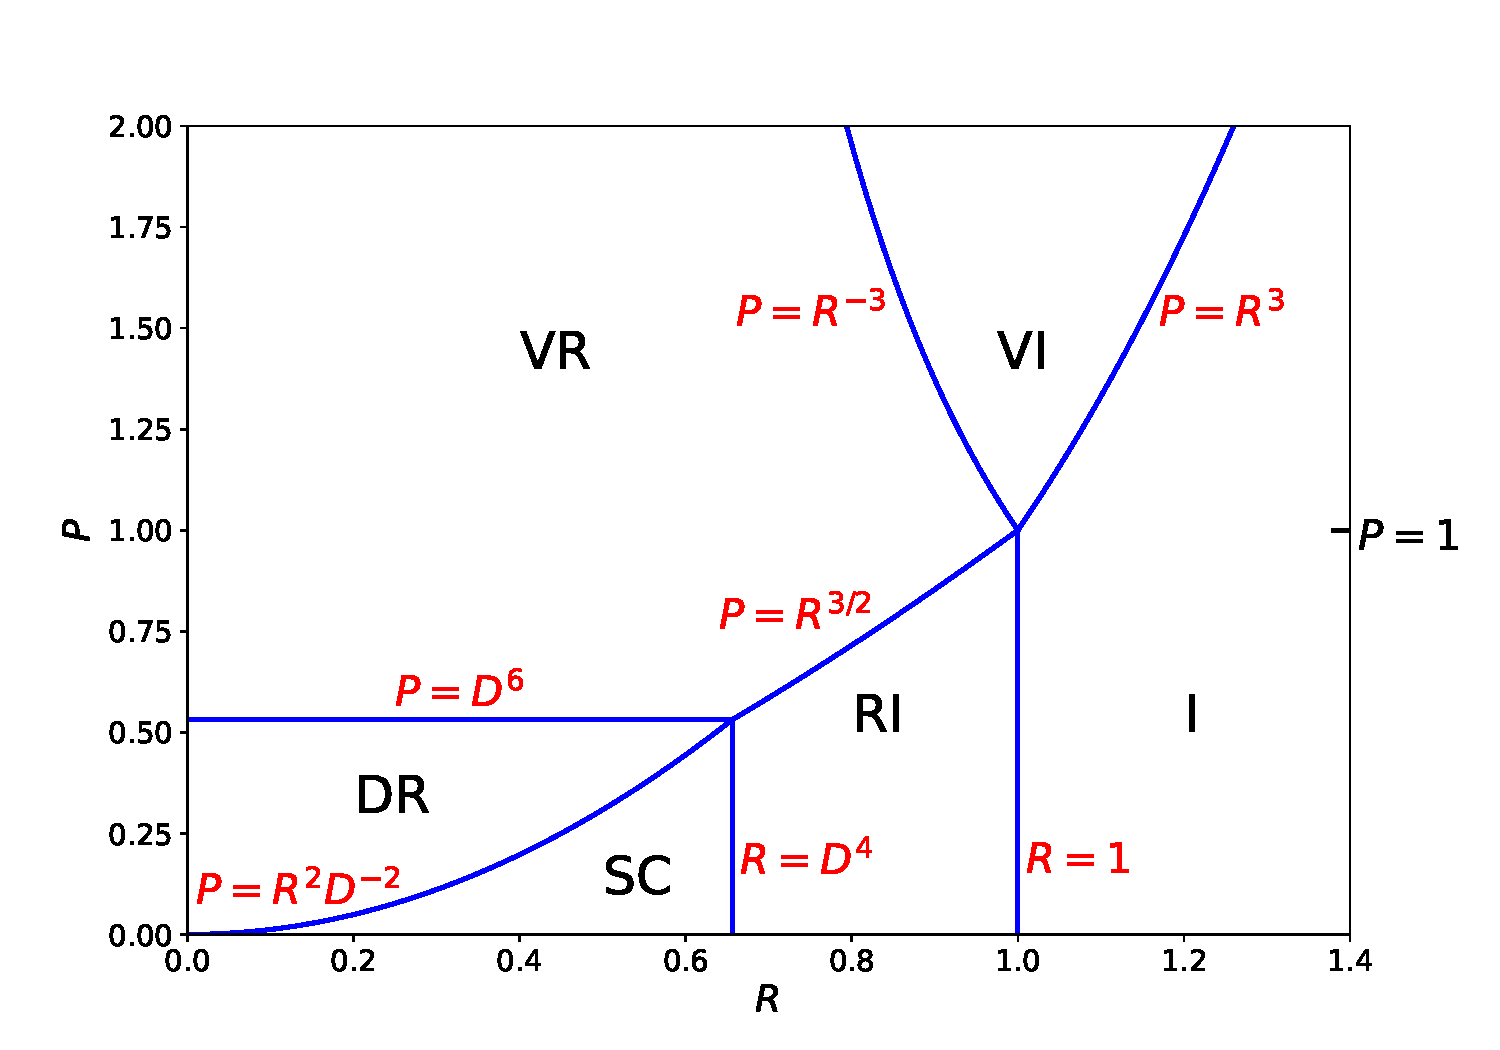
\includegraphics[width=1.\textwidth]{Figure1.pdf}
\caption{Linear resonant plasma response regimes in $R$-$P$ space for the case $D = 0.9$. The various regimes are the diffusive-resisitive (DR), the semi-collisional (SC), the resistive-inertial (RI), the viscous-resistive (VR), the viscous-inertial (VI), and the inertial (I).}\label{f1}
\end{figure}

The {\em semi-collisional}\/ regime is such that
\begin{align}
\hat{\mit\Delta}_s(\hat{g})&= \frac{\pi\,[\hat{g}+{\rm i}\,(Q_E+Q_e)]\,(\hat{g}+{\rm i}\,Q_E)^{1/2}}{D},\label{sc1}\\[0.5ex]
F_s(\hat{g}) &= 1,\\[0.5ex]
\hat{\delta} &= \frac{|{\hat g}+{\rm i}\,Q_E|^{1/2}}{D}.\label{sc3}
\end{align}

The {\em viscous-resistive}\/ regime is such that 
\begin{align}
\hat{\mit\Delta}_s(\hat{g}) &= \frac{6^{2/3}\,\pi\,\Gamma(5/6)}{\Gamma(1/6)}\, [\hat{g}+{\rm i}\,(Q_E+Q_e)]\,P_\varphi^{\,1/6},\label{vr1}\\[0.5ex]
F_s(\hat{g})&= 1,\\[0.5ex]
\hat{\delta} &= P_\varphi^{\,1/6}.\label{vr3}
\end{align}

Finally, the {\em diffusive-resistive}\/ regime is such that
\begin{align}
\hat{\mit\Delta}_s(\hat{g})&= \frac{2\pi\,\Gamma(3/4)}{\Gamma(1/4)}\,\frac{[\hat{g}+{\rm i}\,(Q_E+Q_e)]\,\iota_e^{\,1/4}\,P_\perp^{1/4}}{D^{1/2}},\label{dr1}\\[0.5ex]
F_s(\hat{g}) &= 1,\\[0.5ex]
\hat{\delta} &= \frac{\iota_e^{\,1/4}\,P_\perp^{1/4}}{D^{1/2}}.\label{dr3}
\end{align}
Suppose that $|Q_E|\sim |Q_e|\sim |Q_i|\sim Q$ and $P_\varphi\sim P_\perp\sim P$. Let $R=\sqrt{\hat{g}^2+Q^2}$. The extents of the various
linear resonant response regimes in $R$-$P$ space is illustrated in Figs.~\ref{f1} and \ref{f2}. Note that Fig.~\ref{f2} differs slightly from Fig.~2 in Ref.~\onlinecite{err3} because
we are now demanding equal layer thicknesses at the boundaries between the various response regimes.

\begin{figure}
\centering
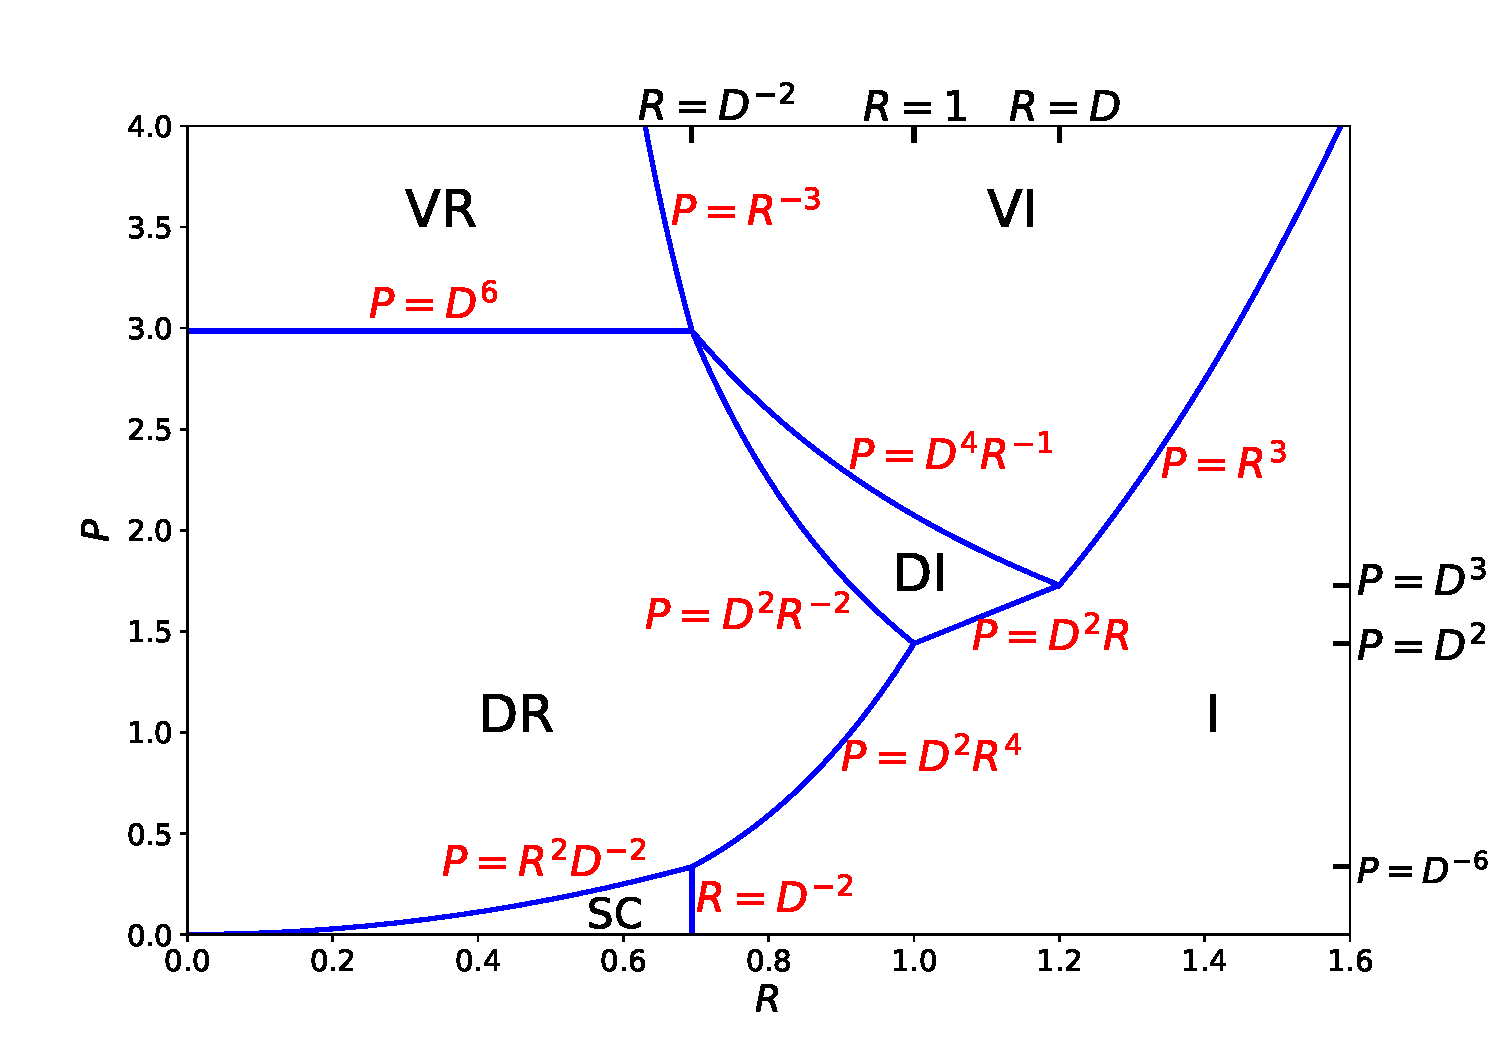
\includegraphics[width=1.\textwidth]{Figure2.pdf}
\caption{Linear resonant plasma response regimes in $R$-$P$ space for the case $D = 1.2$. The various regimes are the diffusive-resisitive (DR), the semi-collisional (SC), the diffusive-inertial (DI), the viscous-resistive (VR), the viscous-inertial (VI), and the inertial (I).}\label{f2}
\end{figure}

\section{Driven Magnetic Reconnection Regimes}\label{regimes}

\subsection{Model RMP}
Suppose that the RMP takes the form 
\begin{equation}\label{e145}
{\mit\Psi}_b(t) = {\mit\Psi}_{b\,0}\left\{\begin{array}{ccc} 0&~~~~&t<0\\[0.5ex]
1&&t\geq 0\end{array}\right..
\end{equation}
In other words, the RMP is switched on suddenly at $t=0$, and thereafter maintains a constant amplitude, ${\mit\Psi}_{b\,0}$. It follows from Eq.~(\ref{psibx}) that
\begin{equation}
\overline{\mit\Psi}_b(\hat{g}) = \frac{{\mit\Psi}_{b\,0}}{\hat{g}}.
\end{equation}
Let
\begin{equation}
{\mit\Psi}_0(\hat{t}) = {\mit\Psi}_\infty\,\hat{\mit\Psi}_0(\hat{t}),
\end{equation}
where
\begin{equation}
{\mit\Psi}_\infty = \frac{E_{sb}\,{\mit\Psi}_{b\,0}}{(-E_{ss})}
\end{equation}
is the reconnected magnetic flux that would be driven at the rational surface in the absence of a helical current sheet at the surface. In other words, ${\mit\Psi}_\infty$ is the maximum possible
time-asymptotic reconnected flux. It follows from Eq.~(\ref{drive}), and the previous three equations,  that
\begin{equation}\label{e29}
\hat{\mit\Psi}_0(\hat{t}) = \frac{1}{2\pi\,{\rm i}}\int_C \frac{F_s(\hat{g})\,{\rm e}^{\,\hat{g}\,\hat{t}}}{\hat{g}\,[{\mit\Sigma}\,\hat{\mit\Delta}_s(\hat{g})+1]}\,d\hat{g},
\end{equation}
where ${\mit\Sigma}= S^{1/3}/(-E_{ss})$. 

In the various non-constant-$\psi$ resonant response regimes (i.e., the inertial, viscous-inertial, and diffusive-inertial regimes), we shall assume that ${\mit\Sigma}\,|\hat{\mit\Delta}_s(g)|\gg 1$, so that 
\begin{equation}\label{ncp}
\hat{\mit\Psi}_0(\hat{t}) \simeq \frac{1}{2\pi\,{\rm i}\,{\mit\Sigma}}\int_C \frac{F_s(\hat{g})\,{\rm e}^{\,\hat{g}\,\hat{t}}}{\hat{g}\,\hat{\mit\Delta}_s(\hat{g})}\,d\hat{g}
\end{equation}
In the various constant-$\psi$ regimes  (i.e., the resistive-inertial, semi-collisional, viscous-resistive, and diffusive-resistive regimes), $F_s\simeq 1$, so that 
\begin{equation}\label{cp}
\hat{\mit\Psi}_0(\hat{t}) \simeq \frac{1}{2\pi\,{\rm i}}\int_C \frac{{\rm e}^{\,\hat{g}\,\hat{t}}}{\hat{g}\,[{\mit\Sigma}\,\hat{\mit\Delta}_s(\hat{g})+1]}\,d\hat{g},
\end{equation}

\subsection{Inertial Reconnection Regime}\label{inertial}
Let $\hat{\mit\Psi}_{I}(\hat{t})$ be the normalized driven magnetic flux in the inertial reconnection regime, and let $\overline{\mit\Psi}_{I}(\hat{g})$ be its Laplace transform.
Equations~(\ref{in1}), (\ref{in2}), and (\ref{ncp}) give
\begin{align}
\overline{\mit\Psi}_{I}(\hat{g}) &= \frac{\epsilon_I}{{\rm i}\,(Q_E+Q_e)}\left[
\frac{1}{\hat{g}}- \frac{1}{\hat{g}+ {\rm i}\,(Q_E+Q_e)}\right]
\frac{1}{(\hat{g}+{\rm i}\,Q_E)^{1/2}\,[\hat{g} + {\rm i}\,(Q_E+Q_i)]^{1/2}},
\end{align}
where
\begin{align}
\epsilon_I = \frac{2}{\pi\,{\mit\Sigma}}.
\end{align}

Now, if
\begin{equation}
\overline{\mit\Psi}_{I}(\hat{g}) = \frac{\overline{H}(\hat{g})}{\hat{g} + a}
\end{equation}
then Eq.~(4.1.20) of Ref.~\onlinecite{ed} yields
\begin{equation}
\hat{\mit\Psi}_{I}(\hat{t}) = \int_0^{\hat{t}}{\rm e}^{\,a\,(\hat{t}'-\hat{t})}\,H(\hat{t}')\,d\hat{t}',
\end{equation}
where $\overline{H}(\hat{g})$ is the Laplace transform of $H(\hat{t})$. 
In the present case,
\begin{align}
\overline{H}(\hat{g}) &= \frac{1}{(\hat{g}+{\rm i}\,Q_E)^{1/2}\,[g +{\rm i}\,(Q_E+Q_i)]^{1/2}}=\frac{1}{(\hat{g}^{\,2}  + \alpha\,\hat{g} + \beta)^{1/2}},
\end{align}
where
$\alpha = {\rm i}\,(2\,Q_E+Q_i)$, and 
$\beta= - Q_E\,(Q_E+Q_i)$.
Note that
\begin{equation}
\beta- \frac{1}{4}\,\alpha^2 = -Q_E\,(Q_E+Q_i) +\frac{1}{4}\,(2\,Q_E+Q_i)^2 = \frac{Q_i^{\,2}}{4}.
\end{equation}
However Eq.~(5.3.34) of Ref.~\onlinecite{ed} gives, 
\begin{align}
H(\hat{t}) &= {\rm e}^{-\alpha\,\hat{t}/2}\,J_0[(\beta-\alpha^2/4)^{1/2}\,\hat{t}]= {\rm e}^{-{\rm i}\,(Q_E+Q_i/2)\,\hat{t}}\,J_0\!\left(\frac{Q_i}{2}\,\hat{t}\right),
\end{align}
where $J_0(z)$ is a Bessel function. 
Thus,
\begin{align}\label{inertialp}
\hat{\mit\Psi}_{I}(\hat{t}) &=\frac{\epsilon_I}{{\rm i}\,(Q_E+Q_e)}
\int_0^{\hat{t}}\left[1-{\rm e}^{\,{\rm i}\,(Q_E+Q_e)\,(\hat{t}'-\hat{t})}\right]
{\rm e}^{-{\rm i}\,(Q_E+Q_i/2)\,\hat{t}'}\,J_0\!\left(\frac{Q_i}{2}\,\hat{t}'\right)d\hat{t}'.
\end{align}

At small $\hat{t}$,
\begin{equation}\label{inertials}
\hat{\mit\Psi}_{I}(\hat{t})\simeq \frac{\epsilon_I\,\hat{t}^{\,2}}{\Gamma(3)},
\end{equation}
where $\Gamma(z)$ is a gamma function.
On the other hand, at large $\hat{t}$,
\begin{align}
\hat{\mit\Psi}_{I}(\hat{t}) &\simeq \frac{\epsilon_I}{{\rm i}\,(Q_E+Q_e)}
\int_0^{\infty}\left[1-{\rm e}^{\,{\rm i}\,(Q_E+Q_e)\,(\hat{t}'-\hat{t})}\right]
{\rm e}^{-{\rm i}\,(Q_E+Q_i/2)\,\hat{t}'}\,J_0\!\left(\frac{Q_i}{2}\,\hat{t}'\right)d\hat{t}'.
\end{align}
But, Eq.~(6.621.4) of Ref.~\onlinecite{grad} yields
\begin{equation}
\int_0^\infty {\rm e}^{-\alpha\,x}\,J_0(\beta\,x)\,dx =\frac{1}{\sqrt{\alpha^2+\beta^2}},
\end{equation}
so
\begin{equation}\label{inertiall}
\hat{\mit\Psi}_{I}(\hat{t})\simeq \frac{\epsilon_I}{{\rm i}\,(Q_E+Q_i)}\left\{
\frac{1}{({\rm i}\,Q_E)^{1/2}\,[{\rm i}\,(Q_E+Q_i)]^{1/2}}- \frac{{\rm e}^{-{\rm i}\,(Q_E+Q_e)\,\hat{t}}}{({\rm i}\,Q_e)^{1/2}\,[{\rm i}\,(Q_e-Q_i)]^{1/2}}\right\}.
\end{equation}

Let $\delta_I =r_s\,S^{-1/3}\,\hat{\delta}_I $ be the radial width of the resonant layer in the inertial reconnection regime. 
In estimating the
layer width, we shall assume that at normalized time $\hat{t}$ the dominant layer response is associated with the following value of the normalized Laplace
transform variable: $\hat{g}=1/\hat{t}$. 
It follows from Eq.~(\ref{in3}) that 
\begin{equation}\label{deltaI}
\hat{\delta}_I(\hat{t})= \frac{1}{\hat{t}}\left(1+Q_E^{\,2}\,\hat{t}^{\,2}\right)^{1/4}\left[1+(Q_E+Q_i)^2\,\hat{t}^{\,2}\right]^{1/4}.
\end{equation}
Thus, at small times, the layer width, which is also the width of the current sheet that  opposes driven magnetic reconnection, decreases in time as $\hat{t}^{-1}$.\cite{hk} However, this decrease eventually stalls, and the
layer width attains a constant value. 

\subsection{Viscous-Inertial Reconnection Regime}
Let $\hat{\mit\Psi}_{VI}(\hat{t})$ be the normalized driven magnetic flux in the viscous-inertial reconnection regime, and let $\overline{\mit\Psi}_{VI}(\hat{g})$ be its Laplace transform.
Equations~(\ref{vi1}), (\ref{vi2}), and (\ref{ncp}) yield
\begin{align}
\overline{\mit\Psi}_{VI}(\hat{g}) =
\frac{ \epsilon_{VI}}{\hat{g}}\,\frac{1}{[\hat{g}+{\rm i}\,(Q_E+Q_e)]^{5/4}},
\end{align}
where
\begin{equation}
\epsilon_{VI} = \frac{1}{\pi^{1/2}\,P_\varphi^{\,1/4}\,{\mit\Sigma}}.
\end{equation}

In this case,
\begin{equation}
\overline{H}(g) = \frac{1}{[\hat{g}+{\rm i}\,(Q_E+Q_e)]^{5/4}},
\end{equation}
so Eq.~(5.4.1) of Ref.~\onlinecite{ed} gives 
\begin{equation}
H(\hat{t}) = \frac{1}{\Gamma(5/4)}\,\hat{t}^{\,1/4}\,{\rm e}^{-{\rm i}\,(Q_E+Q_e)\,\hat{t}}.
\end{equation}
Hence,
\begin{equation}\label{vip}
\hat{\mit\Psi}_{VI}(\hat{t}) =\frac{\epsilon_{VI}}{\Gamma(5/4)}\int_0^{\hat{t}}
\hat{t}'^{\,1/4}\,{\rm e}^{-{\rm i}\,(Q_E+Q_e)\,\hat{t}'}\,d\hat{t}'
\end{equation}

At small $\hat{t}$,
\begin{equation}\label{vis}
\hat{\mit\Psi}_{VI}(\hat{t}) \simeq \frac{\epsilon_{VI}\,\hat{t}^{\,5/4}}{\Gamma(9/4)}.
\end{equation}
On the other hand, at large $\hat{t}$, 
\begin{equation}
\hat{\mit\Psi}_{VI}(\hat{t}) \simeq\frac{\epsilon_{VI}}{\Gamma(5/4)}\int_0^\infty
\hat{t}'^{\,1/4}\,{\rm e}^{-{\rm i}\,(Q_E+Q_e)\,\hat{t}'}\,d\hat{t}'.
\end{equation}
But Eq.~(3.381.5) of Ref.~\onlinecite{grad} yields, 
\begin{equation}
\int_0^\infty x^{\nu-1}\,{\rm e}^{-{\rm i}\,q\,x}\,dx = \frac{\Gamma(\nu)}{({\rm i}\,q)^{\nu}},
\end{equation}
so 
\begin{equation}\label{vil}
\hat{\mit\Psi}_{VI}(\hat{t}) \simeq \frac{\epsilon_{VI}}{[{\rm i}\,(Q_E+Q_e)]^{5/4}}.
\end{equation}

Let $\delta_{VI} =r_s\,S^{-1/3}\,\hat{\delta}_{VI}$ be the radial width of the resonant layer in the viscous-inertial  reconnection regime. 
Equation~(\ref{vi3}) gives 
\begin{equation}
\hat{\delta}_{VI}(\hat{t}) = \frac{1}{\hat{t}^{\,1/4}}\left[1+(Q_E+Q_e)^2\,\hat{t}^{\,2}\right]^{1/8}\,P_\varphi^{\,1/4}.
\end{equation}
Thus, at small times, the layer width decreases in time as $\hat{t}^{-1/4}$. However, this decrease eventually stalls, and the
layer width attains a constant value. 

\subsection{Diffusive-Inertial Reconnection Regime}
Let $\hat{\mit\Psi}_{DI}(\hat{t})$ be the normalized driven magnetic flux in the diffusive-inertial reconnection regime, and let $\overline{\mit\Psi}_{DI}(\hat{g})$ be its Laplace transform.
Equations~(\ref{di1}), (\ref{di2}), and (\ref{ncp}) yield
\begin{align}
\overline{\mit\Psi}_{DI}(\hat{g}) &=\frac{\epsilon_{DI}}{\hat{g}}\,\frac{1}{[\hat{g}+{\rm i}\,(Q_E+Q_e)]^{3/2}},
\end{align}
where
\begin{equation}
\epsilon_{DI} = \frac{2}{\pi}\,\frac{D}{\iota_e^{\,1/2}\,P_\perp^{\,1/2}\,{\mit\Sigma}}.
\end{equation}

In this case,
\begin{equation}
\overline{H}(\hat{g}) = \frac{1}{[\hat{g}+{\rm i}\,(Q_E+Q_e)]^{3/2}},
\end{equation}
so Eq.~(5.4.1.) of Ref.~\onlinecite{ed}  gives
\begin{equation}
H(\hat{t}) = \frac{1}{\Gamma(3/2)}\,\hat{t}^{\,1/2}\,{\rm e}^{-{\rm i}\,(Q_E+Q_e)\,\hat{t}}.
\end{equation}
Hence,
\begin{equation}\label{dip}
\hat{\mit\Psi}_{DI}(\hat{t}) =\frac{\epsilon_{DI}}{\Gamma(3/2)}\int_0^{\hat{t}}
\hat{t}'^{\,1/2}\,{\rm e}^{-{\rm i}\,(Q_E+Q_e)\,\hat{t}'}\,d\hat{t}'
\end{equation}

At small $\hat{t}$,
\begin{equation}\label{dis}
\hat{\mit\Psi}_{DI}(\hat{t}) \simeq \frac{\epsilon_{DI}\,\hat{t}^{\,3/2}}{\Gamma(5/2)}.
\end{equation}
On the other hand, at large $\hat{t}$, 
\begin{equation}
\hat{\mit\Psi}_{DI}(\hat{t}) =\frac{\epsilon_{DI}}{\Gamma(3/2)}\int_0^{\infty}
\hat{t}'^{\,1/2}\,{\rm e}^{-{\rm i}\,(Q_E+Q_e)\,\hat{t}'}\,d\hat{t}'.
\end{equation}
But Eq.~(3.381.5) of Ref.~\onlinecite{grad} yields
\begin{equation}
\int_0^\infty x^{\nu-1}\,{\rm e}^{-{\rm i}\,q\,x}\,dx = \frac{\Gamma(\nu)}{({\rm i}\,q)^{\nu}},
\end{equation}
so 
\begin{equation}\label{dil}
\hat{\mit\Psi}_{DI}(\hat{t}) \simeq \frac{\epsilon_{DI}}{[{\rm i}\,(Q_E+Q_e)]^{3/2}}.
\end{equation}

Let $\delta_{DI} =r_s\,S^{-1/3}\,\hat{\delta}_{DI}$ be the radial width of the resonant layer in the diffusive-inertial reconnection regime. 
Equation~(\ref{di3}) gives 
\begin{equation}
\hat{\delta}_{DI}(\hat{t}) =\frac{1}{\hat{t}^{\,1/2}}\left[1+(Q_E+Q_e)^2\,\hat{t}^{\,2}\right]^{1/4}\iota_e^{\,1/2}\,P_\perp^{\,1/2}.
\end{equation}
Thus, at small times, the layer width decreases in time as $\hat{t}^{-1/2}$. However, this decrease eventually stalls, and the
layer width attains a constant value. 

\subsection{Resistive-Inertial Reconnection Regime}
Let $\hat{\mit\Psi}_{RI}(\hat{t})$ be the normalized driven magnetic flux in the resistive-inertial reconnection regime, and let $\overline{\mit\Psi}_{RI}(\hat{g})$ be its Laplace transform.
Equations~(\ref{ri1}) and (\ref{cp}) yield 
\begin{equation}
\overline{\mit\Psi}_{RI}(\hat{g}) =\frac{\epsilon_{RI}}{\hat{g}}\,\frac{1}{[\hat{g}+{\rm i}\,(Q_E+Q_e)]^{3/4}\,(\hat{g}+{\rm i}\,Q_E)^{1/4}\,[\hat{g}+ {\rm i}\,(Q_E+Q_i)]^{1/4}
+\epsilon_{RI}},
\end{equation}
where
\begin{equation}
\epsilon_{RI}= \frac{\Gamma(1/4)}{2\pi\,\Gamma(3/4)\,{\mit\Sigma}}.
\end{equation}
If we neglect the small parameters $\epsilon_{RI}$ in the denominator then
\begin{equation}
\overline{\mit\Psi}_{RI}(\hat{g}) \simeq\frac{\epsilon_{RI}}{\hat{g}}\,\frac{1}{[\hat{g}+{\rm i}\,(Q_E+Q_e)]^{3/4}\,(\hat{g}+{\rm i}\,Q_E)^{1/4}\,[\hat{g}+ {\rm i}\,(Q_E+Q_i)]^{1/4}}.
\end{equation}

Now, if
\begin{equation}
\overline{\mit\Psi}_{RI}(\hat{g}) \simeq \epsilon_{RI}\,\frac{H(\hat{g})}{\hat{g}}
\end{equation}
then
\begin{equation}
\hat{\mit\Psi}_{RI}(\hat{t}) = \epsilon_{RI}\,\int_0^{\hat{t}}H(\hat{t}')\,d\hat{t'}.
\end{equation}
Furthermore, if
\begin{equation}
\overline{H}(\hat{g}) = \overline{H}_1(\hat{g})\,\overline{H}_2(\hat{g})
\end{equation}
then
\begin{equation}
H(\hat{t})=\int_0^{\hat{t}}H_1(\hat{t}')\,H_2(\hat{t}-\hat{t}')\,d\hat{t}'.
\end{equation}
It follows that
\begin{equation}
\hat{\mit\Psi}_{RI}(\hat{t}) = \epsilon_{RI}\int_0^{\hat{t}}\left[\int_0^{\hat{t}'}
H_1(\hat{t}'')\,H_2(\hat{t}'-\hat{t}'')\,d\hat{t}''\right]d\hat{t'}.
\end{equation}

In the present case
\begin{align}
\overline{H}_1(\hat{g}) &= \frac{1}{(\hat{g}+{\rm i}\,Q_E)^{1/4}\,[\hat{g}+ {\rm i}\,(Q_E+Q_i)]^{1/4}},\\[0.5ex]
\overline{H}_2(\hat{g}) &= \frac{1}{[\hat{g}+{\rm i}\,(Q_E+Q_e)]^{3/4}},
\end{align}
so Eqs.~(5.4.5) and (5.4.1) of Ref.~\onlinecite{ed}, and (9.6.3) of Ref.~\onlinecite{abram}, yield 
\begin{align}
H_1(\hat{t}) &= \frac{\pi^{1/2}}{\Gamma(1/4)}\,Q_i^{\,1/4}\,\hat{t}^{-1/4}\,{\rm e}^{-{\rm i}\,(Q_E+Q_i/2)\,\hat{t}}\,J_{-1/4}\!\left(\frac{Q_i}{2}\,\hat{t}\right),\\[0.5ex]
H_2(\hat{t})&= \frac{1}{\Gamma(3/4)}\,\hat{t}^{-1/4}\,{\rm e}^{-{\rm i}\,(Q_E+Q_e)\,\hat{t}}.
\end{align}
Note that
$\Gamma(1/4)\,\Gamma(3/4) = \sqrt{2}\,\pi$.
Thus,
\begin{align}\label{rip}
\hat{\mit\Psi}_{RI}(\hat{t}) &= \frac{\epsilon_{RI}\,Q_i^{\,1/4}}{\sqrt{2\pi}}\int_0^{\hat{t}}{\rm e}^{-{\rm i}\,(Q_E+Q_e)\,\hat{t}'}\left[
\int_0^{\hat{t}'}(\hat{t}'-\hat{t}'')^{-1/4}\,\hat{t}''^{-1/4}
{\rm e}^{\,{\rm i}\,(Q_e-Q_i/2)\,\hat{t}''}\,J_{-1/4}\!\left(\frac{Q_i}{2}\,\hat{t}''\right)d\hat{t}''\right]d\hat{t}'.
\end{align}

At small $\hat{t}$, Eq.~(9.1.10) of Ref.~\onlinecite{abram} gives
\begin{equation}
J_{-1/4}\!\left(\frac{Q_i}{2}\,\hat{t}\right)\simeq\frac{\sqrt{2}\,Q_i^{-1/4}\,\hat{t}^{-1/4}}{\Gamma(3/4)},
\end{equation}
so
\begin{equation}
\hat{\mit\Psi}_{RI}(\hat{t})\simeq \frac{\epsilon_{RI}}{\sqrt{\pi}\,\Gamma(3/4)}
\int_0^{\hat{t}}\left[\int_0^{\hat{t}'}(\hat{t}'-\hat{t}'')^{-1/4}\,\hat{t}''^{-1/2}\,d\hat{t}''\right]d\hat{t}'.
\end{equation}
But,
\begin{equation}
\int_0^{\hat{t}'}(\hat{t}'-\hat{t}'')^{-1/4}\,\hat{t}''^{-1/2}\,d\hat{t}''=\hat{t}'^{\,1/4}\int_0^1(1-x)^{-1/4}\,x^{-1/2}\,dx,
\end{equation}
and Eqs.~(6.2.1) and (6.2.2) of Ref.~\onlinecite{abram} yield
\begin{equation}
\int_0^1(1-x)^{-1/4}\,x^{-1/2}\,dx =\frac{\Gamma(1/2)\,\Gamma(3/4)}{\Gamma(5/4)},
\end{equation}
so
\begin{equation}\label{ris}
{\mit\Psi}_{RI}(\hat{t})\simeq \frac{\epsilon_{RI}\,\hat{t}^{\,5/4}}{\Gamma(9/4)}.
\end{equation}

On the other hand, at large $\hat{t}$, 
\begin{align}
\hat{\mit\Psi}_{RI}(\hat{t}) &\simeq \frac{\epsilon_{RI}\,Q_i^{\,1/4}}{\sqrt{2\pi}}\int_0^{\infty}{\rm e}^{-{\rm i}\,(Q_E+Q_e)\,\hat{t}'}
\left[\int_0^{\hat{t}'}(\hat{t}'-\hat{t}'')^{-1/4}\,\hat{t}''^{-1/4}
{\rm e}^{\,{\rm i}\,(Q_e-Q_i/2)\,\hat{t}''}\,J_{-1/4}\!\left(\frac{Q_i}{2}\,\hat{t}''\right)d\hat{t}''\right]d\hat{t}',
\end{align}
so
\begin{align}
\hat{\mit\Psi}_{RI}(\hat{t}) &\simeq \frac{\epsilon_{RI}\,Q_i^{\,1/4}}{\sqrt{2\pi}}
\int_0^\infty\left[\int_{\hat{t}''}^\infty(\hat{t'}-\hat{t}'')^{-1/4}\,{\rm e}^{-{\rm i}\,(Q_E+Q_e)\,\hat{t}'}\,d\hat{t}'\right]
 \hat{t}''^{-1/4}\,{\rm e}^{\,{\rm i}\,(Q_e-Q_i/2)\,\hat{t}''}\,J_{-1/4}\!\left(\frac{Q_i}{2}\,\hat{t}''\right)\,d\hat{t}''.
\end{align}
But,
\begin{align}
\int_{\hat{t}''}^\infty(\hat{t'}-\hat{t}'')^{-1/4}\,{\rm e}^{-{\rm i}\,(Q_E+Q_e)\,\hat{t}'}\,d\hat{t}'={\rm e}^{-{\rm i}\,(Q_E+Q_e)\,\hat{t}''} \int_0^\infty
x^{-1/4}\,{\rm e}^{-{\rm i}\,(Q_E+Q_e)\,x}\,dx,
\end{align}
and Eq.~(3.381.5) of Ref.~\onlinecite{grad} gives
\begin{equation}
\int_0^\infty x^{\nu-1}\,{\rm e}^{-{\rm i}\,q\,x}\,dx = \frac{\Gamma(\nu)}{({\rm i}\,q)^{\nu}},
\end{equation}
so 
\begin{equation}
\int_{\hat{t}''}^\infty (\hat{t'}-\hat{t}'')^{-1/4}\,{\rm e}^{-{\rm i}\,(Q_E+Q_e)\,\hat{t}'}\,d\hat{t}'={\rm e}^{-{\rm i}\,(Q_E+Q_e)\,\hat{t}''} \, \frac{\Gamma(3/4)}{[{\rm i}\,(Q_E+Q_e)]^{3/4}}.
\end{equation}
It follows that
\begin{align}
\hat{\mit\Psi}_{RI}(\hat{t})&= \frac{\epsilon_{RI}\,Q_i^{\,1/4}}{\sqrt{2\pi}}\,\frac{\Gamma(3/4)}{[{\rm i}\,(Q_E+Q_e)]^{3/4}}
\int_0^\infty \hat{t}''^{-1/4}\,{\rm e}^{-{\rm i}\,(Q_E+Q_i/2)\,\hat{t''}}\,J_{-1/4}\left(\frac{Q_i}{2}\,\hat{t}''\right)d\hat{t}''.
\end{align}
But, Eq.~(6.623.1) of Ref.~\onlinecite{grad}  yields 
\begin{align}
&\int_0^\infty \hat{t}''^{-1/4}\,{\rm e}^{-{\rm i}\,(Q_E+Q_i/2)\,\hat{t''}}\,J_{-1/4}\!\left(\frac{Q_i}{2}\,\hat{t}''\right)d\hat{t}'' 
= \frac{(Q_i)^{-1/4}\,\Gamma(1/4)}{\sqrt{\pi}\,({\rm i}\,Q_E)^{1/4}\,[{\rm i}\,(Q_E+Q_i)]^{1/4}}.
\end{align}
Now, Eq.~(6.1.17) of Ref.~\onlinecite{abram} gives
$\Gamma(3/4)\,\Gamma(1/4)= \sqrt{2}\,\pi$,
so
\begin{equation}\label{ril}
\hat{\mit\Psi}_{RI}(\hat{t})\simeq 
\frac{\epsilon_{RI}}{[{\rm i}\,(Q_E+Q_e)]^{3/4}\,({\rm i}\,Q_E)^{1/4}\,[{\rm i}\,(Q_E+Q_i)]^{1/4}}.
\end{equation}

Let $\delta_{RI} =r_s\,S^{-1/3}\,\hat{\delta}_{RI}$ be the radial width of the resonant layer in the resistive-inertial reconnection regime. Equation~(\ref{ri3})
yields 
\begin{equation}
\hat{\delta}_{RI}(\hat{t}) =\frac{1}{\hat{t}^{\,1/4}}\,\frac{\left(1+ Q_E^{\,2}\,\hat{t}^{\,2}\right)^{1/8}\left[1+(Q_E+Q_i)^2\,\hat{t}^{\,2}\right]^{1/8}}
{\left[1+(Q_E+Q_e)^2\,\hat{t}^{\,2}\right]^{1/8}}.
\end{equation}
Thus, at small times, the layer width decreases in time as $\hat{t}^{-1/4}$. However, this decrease eventually stalls, and the
layer width attains a constant value. 

\subsection{Semi-Collisional Reconnection Regime}
Let $\hat{\mit\Psi}_{SC}(\hat{t})$ be the normalized driven magnetic flux in the semi-collisional reconnection regime, and let $\overline{\mit\Psi}_{SC}(\hat{g})$ be its Laplace transform.
Equations~(\ref{sc1}) and (\ref{cp}) yield 
\begin{equation}
\overline{\mit\Psi}_{SC}(\hat{g}) =\frac{\epsilon_{SC}}{\hat{g}}\,\frac{1}{[\hat{g}+ {\rm i}\,(Q_E+Q_e)]\,(\hat{g}+{\rm i} \,Q_E)^{1/2}
+\epsilon_{SC}},
\end{equation}
where
\begin{equation}
\epsilon_{SC}= \frac{D}{\pi\,{\mit\Sigma}}.
\end{equation}
If we neglect the small parameter $\epsilon_{SC}$ in the denominator then
\begin{equation} 
\overline{\mit\Psi}_{SC}(\hat{g}) \simeq \frac{\epsilon_{SC}}{\hat{g}}\,\frac{1}{[\hat{g}+ {\rm i}\,(Q_E+Q_e)]\,(g+{\rm i} \,Q_E)^{1/2}},
\end{equation}
giving 
\begin{equation}
\overline{\mit\Psi}_{SC}(\hat{g}) \simeq \frac{\epsilon_{SC}}{{\rm i}\,(Q_E+Q_e)}
\left[\frac{1}{\hat{g}}- \frac{1}{\hat{g}+ {\rm i}\,(Q_E+Q_e)}\right]\frac{1}{(\hat{g}+{\rm i} \,Q_E)^{1/2}}.
\end{equation}
In this case, 
\begin{equation}
\overline{H}(\hat{g}) = \frac{1}{(\hat{g}+{\rm i}\,Q_E)^{1/2}},
\end{equation}
so Eq.~(5.4.1) of Ref.~\onlinecite{ed} yields
\begin{equation}
H(\hat{t}) = \frac{1}{\Gamma(1/2)}\,\hat{t}^{-1/2}\,{\rm e}^{-{\rm i}\,Q_E\,\hat{t}}.
\end{equation}
Hence,
\begin{align}\label{scpx}
\hat{\mit\Psi}_{SC}(\hat{t}) &= \frac{\epsilon_{SC}}{\Gamma(1/2)\,{\rm i}\,(Q_E+Q_e)} \int
_0^{\hat{t}}\left[1-{\rm e}^{\,{\rm i}\,(Q_E+Q_e)\,(\hat{t}'-\hat{t})}\right]
\hat{t}'^{-1/2}\,{\rm e}^{-{\rm i}\,Q_E\,\hat{t'}}\,d\hat{t}'.
\end{align}

At small $\hat{t}$, 
\begin{align}\label{scs}
\hat{\mit\Psi}_{SC}(\hat{t}) &= \frac{\epsilon_{SC}\,\hat{t}^{\,3/2}}{\Gamma(5/2)}.
\end{align}
On the other hand, at large $\hat{t}$, 
\begin{align}
\hat{\mit\Psi}_{SC}(\hat{t}) &= \frac{\epsilon_{SC}}{\Gamma(1/2)\,{\rm i}\,(Q_E+Q_e)} \int
_0^{\infty}\left[1-{\rm e}^{\,{\rm i}\,(Q_E+Q_e)\,(\hat{t}'-\hat{t})}\right]
\hat{t}'^{-1/2}\,{\rm e}^{-{\rm i}\,Q_E\,\hat{t'}}\,d\hat{t}'.
\end{align}
But Eq.~(3.381.5) of Ref.~\onlinecite{grad} gives
\begin{equation}
\int_0^\infty x^{\nu-1}\,{\rm e}^{-{\rm i}\,q\,x}\,dx = \frac{\Gamma(\nu)}{({\rm i}\,q)^{\nu}},
\end{equation}
It follows that
\begin{equation}\label{scl}
\hat{\mit\Psi}_{SC}(\hat{t}) = \frac{\epsilon_{SC}}{{\rm i}\,(Q_E+Q_e)}
\left[\frac{1}{({\rm i}\,Q_E)^{1/2}} - \frac{{\rm e}^{-{\rm i}\,(Q_E+Q_e)\,\hat{t}}}{(-{\rm i}\,Q_e)^{1/2}}\right].
\end{equation}

Let $\delta_{SC} =r_s\,S^{-1/3}\,\hat{\delta}_{SC}$ be the radial width of the resonant layer in the semi-collisional regime. 
Equation~(\ref{sc3}) yields
\begin{equation}
\hat{\delta}_{SC}(\hat{t}) = \frac{1}{\hat{t}^{\,1/2}}\left(1+Q_E^{\,2}\,\hat{t}^{\,2}\right)^{1/4}\,D^{-1}.
\end{equation}
Thus, at small times, the layer width decreases in time as $\hat{t}^{-1/2}$. However, this decrease eventually stalls, and the
layer width attains a constant value. 

\subsection{Viscous-Resistive Reconnection Regime}
Let $\hat{\mit\Psi}_{VR}(\hat{t})$ be the normalized driven magnetic flux in the viscous-resistive reconnection regime, and let $\overline{\mit\Psi}_{VR}(\hat{g})$ be its Laplace transform.
Equations~(\ref{vr1}) and (\ref{cp}) give
\begin{equation}
\overline{\mit\Psi}_{VR}(\hat{g}) =\frac{\epsilon_{VR}}{\hat{g}}\,\frac{1}{[\hat{g}+ {\rm i}\,(Q_E+Q_e)]+\epsilon_{VR}},
\end{equation}
where
\begin{equation}
\epsilon_{VR} = \frac{\Gamma(1/6)}{6^{2/3}\,\pi\,\Gamma(5/6)}\,\frac{1}{P_\varphi^{\,1/6}\,{\mit\Sigma}}.
\end{equation}
Thus,
\begin{align}
\overline{\mit\Psi}_{VR}(\hat{g}) &= 
\frac{\epsilon_{VR}}{{\rm i}\,(Q_E+Q_e)+\epsilon_{VR}}\left(\frac{1}{\hat{g}} - \frac{1}{\hat{g} +[ {\rm i}\,(Q_E+Q_e)+\epsilon_{VR}]}\right),
\end{align}
giving
\begin{align}\label{vrp}
\hat{\mit\Psi}_{VR}(\hat{t}) &= \frac{\epsilon_{VR}}{{\rm i}\,(Q_E+Q_e)+\epsilon_{VR}}\left(1 - {\rm e}^{- [{\rm i}\,(Q_E+Q_e)+\epsilon_{VR}]\,\hat{t}}\right).
\end{align}

At small $\hat{t}$,
\begin{align}\label{vrs}
\hat{\mit\Psi}_{VR}(\hat{t}) &\simeq \frac{\epsilon_{VR}\,\hat{t}}{\Gamma(2)}.
\end{align}
On the other hand, at large $\hat{t}$, 
\begin{align}\label{vrl}
\hat{\mit\Psi}_{VR}(\hat{t}) &\simeq 
\frac{\epsilon_{VR}}{{\rm i}\,(Q_E+Q_e)+\epsilon_{VR}}.
\end{align}

Let $\delta_{VR} =r_s\,S^{-1/3}\,\hat{\delta}_{VR}$ be the radial width of the resonant layer in the viscous-resistive reconnection regime. 
Equation~(\ref{vr3}) yields
\begin{equation}
\hat{\delta}_{VR}(\hat{t}) = P_\varphi^{\,1/6}.
\end{equation}
Thus, the layer width is independent of time. 

\subsection{Diffusive-Resistive Reconnection Regime}\label{diffusive}
Let $\hat{\mit\Psi}_{DR}(\hat{t})$ be the normalized driven magnetic flux in the diffusive-resistive reconnection regime, and let $\overline{\mit\Psi}_{DR}(\hat{g})$ be its Laplace transform.
 Equations~(\ref{dr1}) and (\ref{cp}) yield 
 \begin{equation}
\overline{\mit\Psi}_{DR}(\hat{g}) =\frac{\epsilon_{DR}}{\hat{g}}\,\frac{1}
{[\hat{g}+ {\rm i}\,(Q_E+Q_e)]+\epsilon_{DR}},
\end{equation}
where
\begin{equation}
\epsilon_{DR} = \frac{\Gamma(1/4)}{2\pi\,\Gamma(3/4)}\,\frac{D^{1/2}}{\iota_e^{\,1/4}\,P_\perp^{\,1/4}\,{\mit\Sigma}}.
\end{equation}
Thus,
\begin{align}
\overline{\mit\Psi}_{DR}(\hat{g}) &=
\,\frac{\epsilon_{DR}}{{\rm i}\,(Q_E+Q_e)+\epsilon_{DR}}\left(\frac{1}{\hat{g}} - \frac{1}{\hat{g} + [{\rm i}\,(Q_E+Q_e)+\epsilon_{DR}]}\right),
\end{align}
yielding 
\begin{align}\label{drp}
\hat{\mit\Psi}_{DR}(\hat{t}) &=
\frac{\epsilon_{DR}}{{\rm i}\,(Q_E+Q_e)+\epsilon_{DR}}\left(1 - {\rm e}^{- [{\rm i}\,(Q_E+Q_e)+\epsilon_{DR}]\,\hat{t}}\right).
\end{align}

At small $\hat{t}$,
\begin{align}\label{drs}
{\mit\Psi}_{DR}(\hat{t}) &\simeq\frac{\epsilon_{DR}\,\hat{t}}{\Gamma(2)}.
\end{align}
On the other hand, at large $\hat{t}$, 
\begin{align}\label{drl}
\hat{\mit\Psi}_{DR}(\hat{t}) &\simeq 
\frac{\epsilon_{DR}}{{\rm i}\,(Q_E+Q_e)+\epsilon_{DR}}.
\end{align}

Let $\delta_{DR} =r_s\,S^{-1/3}\,\hat{\delta}_{DR}$ be the radial width of the resonant layer in the diffusive-resistive reconnection regime. 
Equation~(\ref{dr3}) gives 
\begin{equation}
\hat{\delta}_{DR}(\hat{t}) = \frac{\iota_e^{\,1/4}\,P_\perp^{1/4}}{D^{1/2}}.
\end{equation}
Thus, the layer width is independent of time. 

\begin{figure}[t]
\centering
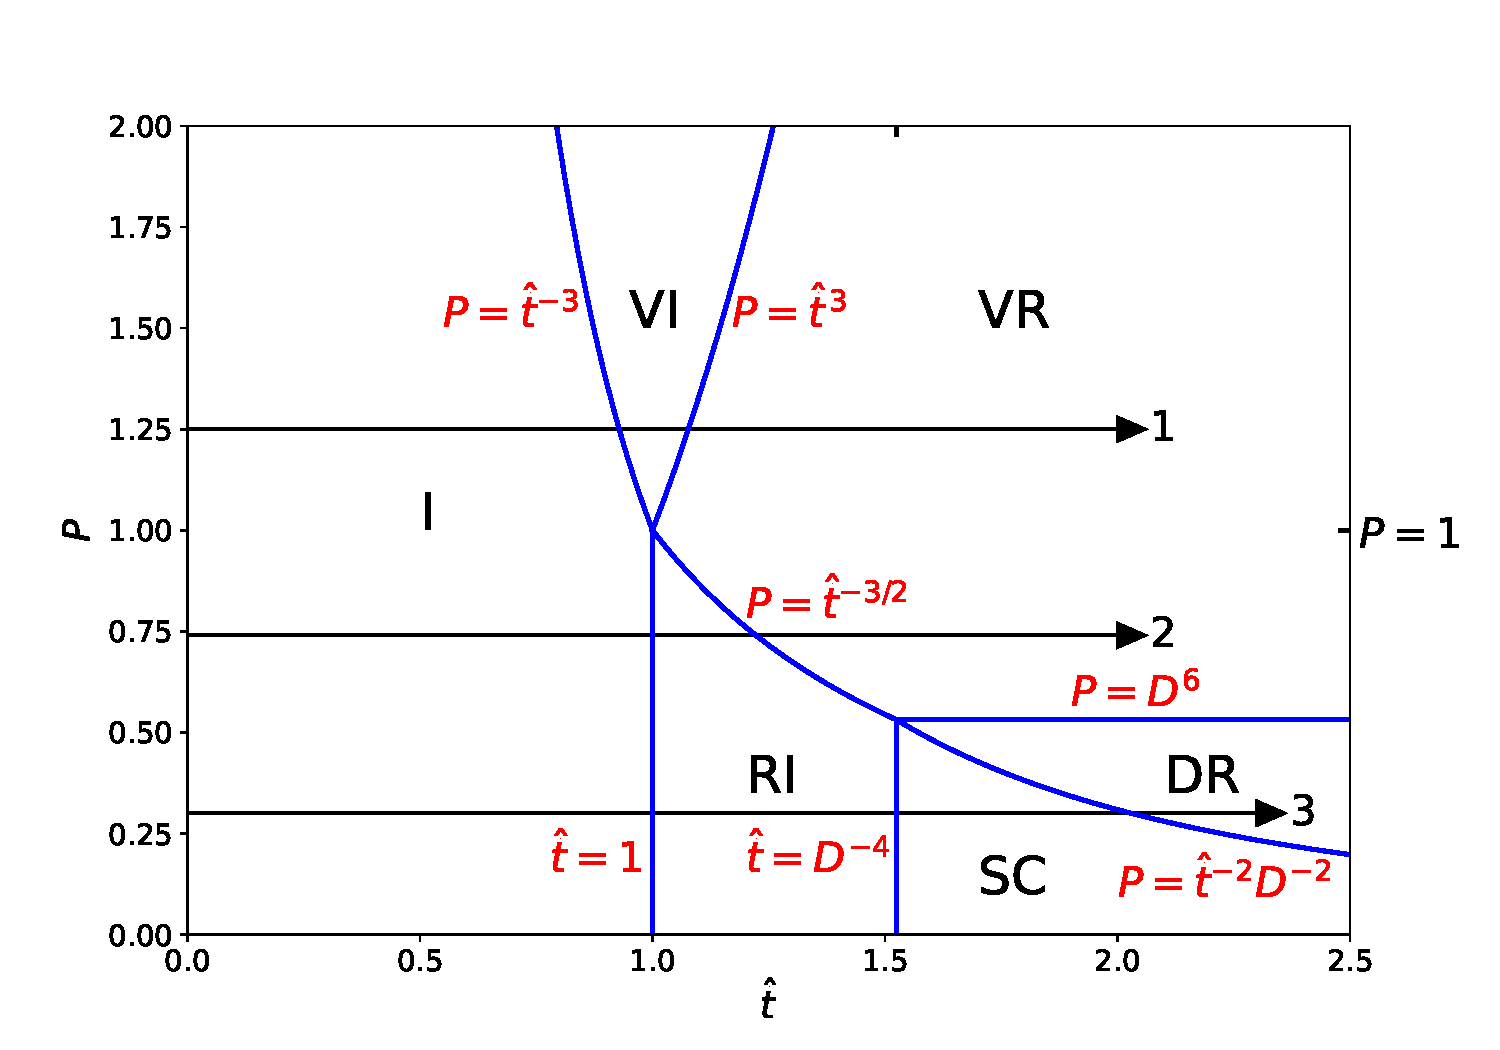
\includegraphics[width=1.\textwidth]{Figure3.pdf}
\caption{Trajectory of the Fourier-Laplace transformed response of a resonant layer to a resonant magnetic perturbation in $\hat{t}$-$P$ space for the case $D=0.9$. The various regimes are the diffusive-resistive (DR), the semi-collisional (SC), the resistive-inertial (RI), the viscous-resistive (VR), the viscous-inertial (VI), and the inertial (I). }\label{f3}
\end{figure}

\section{Reconnection Scenarios}\label{scenarios}
The layer widths calculated in Sects.~\ref{inertial}--\ref{diffusive} allow us to determine how the driven magnetic flux at the rational surface
evolves through the various reconnection regimes as a function of time. This evolution is illustrated in Figs.~\ref{f3} and \ref{f4}.

Consider reconnection scenario 1, which corresponds to the horizontal lines labelled 1 in Figs.~\ref{f3} and \ref{f4}. 
This scenario holds when $D<1$ and $P>1$, or when  $D>1$ and $P>D^{\,6}$. 
The plasma in the resonant layer starts off in the inertial regime, passes into the viscous-inertial regime if and when  $\hat{\delta}_I(\hat{t})=\hat{\delta}_{VI}(\hat{t})$,
and passes into the viscous-resistive regime if and when $\hat{\delta}_{VI}(\hat{t})=\hat{\delta}_{VR}(\hat{t})$. 
Thus, the normalized reconnected magnetic flux is specified by $\hat{\mit\Psi}_{I}(\hat{t})$ in the first time interval,
by $\hat{\mit\Psi}_{VI}(\hat{t})$ in the second interval, and by $\hat{\mit\Psi}_{VR}(\hat{t})$ in the third. Analogous statements can be
made for the other reconnection scenarios.  

Consider reconnection scenario 2, which corresponds to the horizontal line labelled 2 in Fig.~\ref{f3}. 
This scenario holds when $D<1$ and $D^{\,6}<P< 1$. The plasma in the resonant layer starts off in the inertial regime, passes into the resistive-inertial regime if and when $\hat{\delta}_I(\hat{t})=\hat{\delta}_{RI}(\hat{t})$,
and passes into the viscous-resistive regime if and when $\hat{\delta}_{RI}(\hat{t})=\hat{\delta}_{VR}(\hat{t})$. 

Consider reconnection scenario 3, which corresponds to the horizontal line labelled 3 in Fig.~\ref{f3}. 
This scenario holds when $D<1$ and $P<D^{\,6}$. 
The plasma in the resonant layer starts off in the inertial regime, passes into the resistive-inertial regime if and when $\hat{\delta}_I(\hat{t})=\hat{\delta}_{RI}(\hat{t})$, passes into the semi-collisional regime if and when $\hat{\delta}_{RI}(\hat{t})=\hat{\delta}_{SC}(\hat{t})$, and passes into the
viscous-resistive regime if and when $\hat{\delta}_{SC}(\hat{t})=\hat{\delta}_{RI}(\hat{t})$.

Consider reconnection scenario 4, which corresponds to the horizontal line labelled 4 in Fig.~\ref{f4}. 
This scenario holds when $D>1$ and $D^{\,3} < P<D^{\,6}$. 
The plasma in the resonant layer starts off in the inertial regime, passes into the viscous-inertial regime if and when $\hat{\delta}_I(\hat{t})=\hat{\delta}_{VI}(\hat{t})$, passes into the diffusive-inertial regime if and when $\hat{\delta}_{VI}(\hat{t})=\hat{\delta}_{DR}(\hat{t})$, and passes into the
diffusive-resistive regime if and when $\hat{\delta}_{DI}(\hat{t})=\hat{\delta}_{DR}(\hat{t})$.

Consider reconnection scenario 5, which corresponds to the horizontal line labelled 5 in Fig.~\ref{f4}. 
This scenario holds when $D>1$ and $D^{\,2} < P<D^{\,5}$. 
The plasma in the resonant layer starts off in the inertial regime, passes into the diffusive-inertial regime if and when $\hat{\delta}_I(\hat{t})=\hat{\delta}_{DI}(\hat{t})$, and passes into the
diffusive-resistive regime if and when $\hat{\delta}_{DI}(\hat{t})=\hat{\delta}_{DR}(\hat{t})$.

Consider reconnection scenario 6, which corresponds to the horizontal line labelled 6 in Fig.~\ref{f4}. 
This scenario holds when $D>1$ and $D^{\,-6} < P<D^{\,2}$. 
The plasma in the resonant layer starts off in the inertial regime,  and passes into the
diffusive-resistive regime if and when $\hat{\delta}_{I}(\hat{t})=\hat{\delta}_{DR}(\hat{t})$.

Finally, consider reconnection scenario 7, which corresponds to the horizontal line labelled 7 in Fig.~\ref{f4}. 
This scenario holds when $D>1$ and $P<D^{\,-6}$. 
The plasma in the resonant layer starts off in the inertial regime, passes into the semi-collisional regime if and when $\hat{\delta}_I(\hat{t})=\hat{\delta}_{SC}(\hat{t})$, and passes into the
diffusive-resistive regime if and when $\hat{\delta}_{SC}(\hat{t})=\hat{\delta}_{DR}(\hat{t})$.

\begin{figure}
\centering
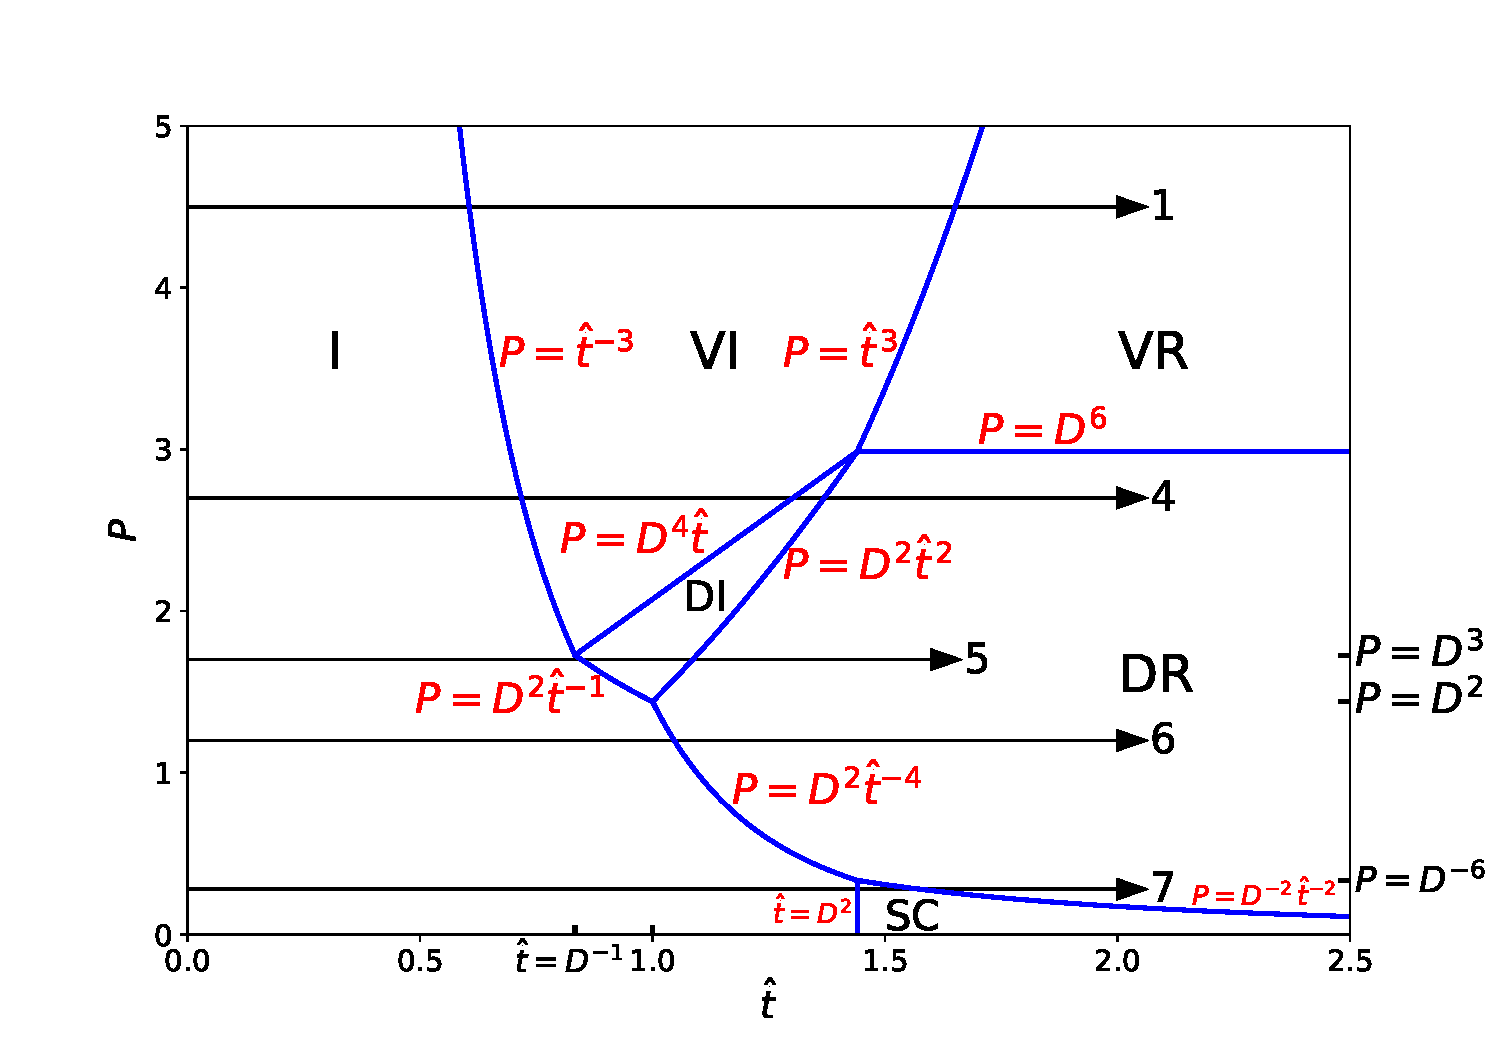
\includegraphics[width=1.\textwidth]{Figure4.pdf}
\caption{Trajectory of the Fourier-Laplace transformed response of a resonant layer to a resonant magnetic perturbation  in $\hat{t}$-$P$ space for the case $D=1.2$. The various regimes are the diffusive-resistive (DR), the semi-collisional (SC), the diffusive-inertial (DI), the viscous-resistive (VR), the viscous-inertial (VI), and the inertial (I).}\label{f4}
\end{figure}

\begin{table}[t]
\begin{tabular}{cccccccc}\hline
Scenario & ~${\mit\Sigma}$~ & ~$Q_E$~ & ~$Q_e$~ & ~$Q_i$~ & ~~$D$~ & ~$P_\perp$~ & ~$P_\varphi$\\[0.5ex]\hline
1 & 10 & 0.1 & 1.0 & $-1.0$ & 1.2 &  5.0 & 5.0\\[0.5ex]
3 & 10 & 0.1 & 1.0 &$-1.0$ & 0.9 & 0.25 & 0.25\\[0.5ex]
5 & 10 & 0.1 & 1.0  &$-1.0$ & 1.2 & 1.728 & 1.728
\end{tabular}
\caption{Normalized layer parameters used in simulations of various reconnection scenarios.}\label{t1}
\end{table}

\section{Simulations}
\subsection{Introduction}
We can calculate the normalized driven reconnected magnetic flux at the rational surface, $\hat{\mit\Psi}_0$, as a function of normalized time, $\hat{t}$, by one of two alternative  methods.  The first solution  method,
which is exact,  involves numerically 
evaluating the contour integral (\ref{e29}): i.e., 
\begin{equation}
\hat{\mit\Psi}_0(\hat{t}) = \frac{1}{2\pi\,{\rm i}}\int_{\sigma-{\rm i}\,\infty}^{\sigma+{\rm i}\,\infty}\frac{F_s(\hat{g})\,{\rm e}^{\,\hat{g}\,\hat{t}}}{\hat{g}\,[{\mit\Sigma}\,\hat{\mit\Delta}_s(\hat{g})+1]}\,d\hat{g}.
\end{equation}
Here, the layer quantities $\hat{\mit\Delta}_s(\hat{g})$ and $F_s(\hat{g})$ must be calculated numerically by means of the two-step method described in Appendix~\ref{appd}. In all of the calculations described in this paper, 
 $\sigma = 0.1$. (We have confirmed that the results of the calculation  are independent of the value of $\sigma$, provided that it is positive.) The second solution method,
 which is only approximate,  but much less time consuming, involves evaluating the closed-form analytic expressions (\ref{inertialp}),
(\ref{vip}), (\ref{dip}), (\ref{rip}), (\ref{scpx}), (\ref{vrp}), and (\ref{drp}) for $\hat{\mit\Psi}_0(\hat{t})$ in each of the seven reconnection regimes. 

\begin{figure}[t]
\centering
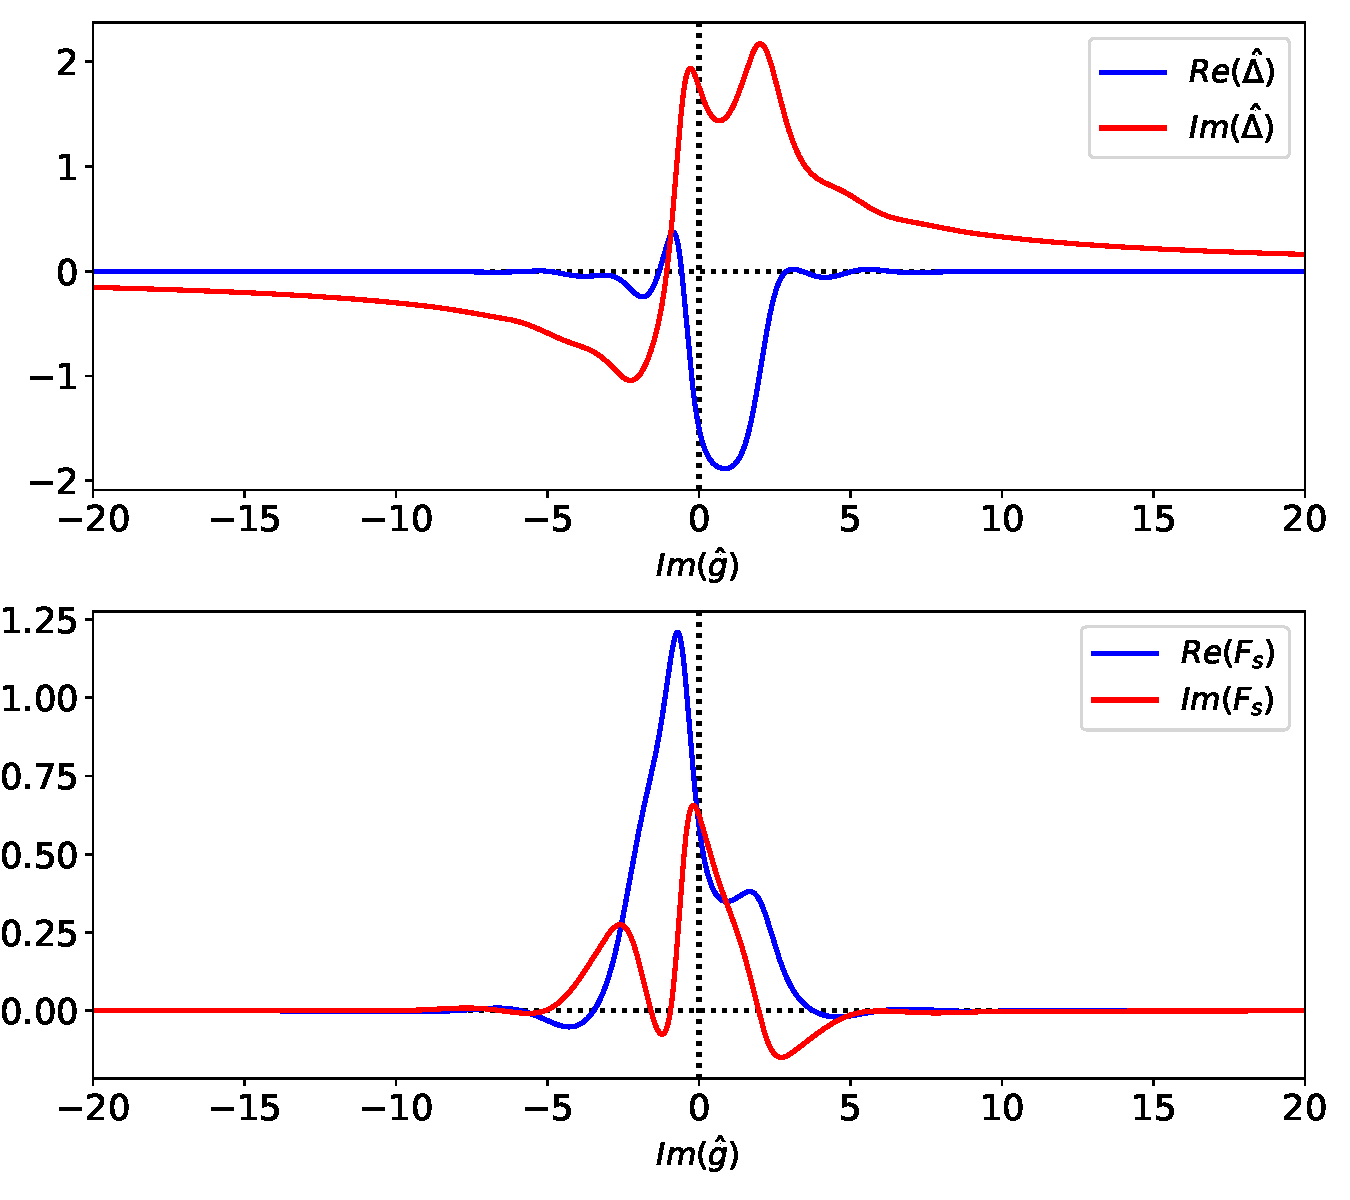
\includegraphics[width=0.8\textwidth]{Figure5.pdf}
\caption{The layer quantities $\hat{\mit\Delta}_s(\hat{g})$ and $F_s(\hat{g})$ calculated numerically along the Bromwich contour in Reconnection Scenario 1.}\label{f5}
\end{figure}

\subsection{Reconnection Scenario 1}
Consider Reconnection Scenario 1, which is illustrated in Figs.~\ref{f3} and \ref{f4}.  The normalized layer parameters used to access this regime are listed  in Table~\ref{t1}. 

Figure~\ref{f5} shows
the layer quantities $\hat{\mit{\Delta}}_s(\hat{g})$ and $F_s(\hat{g})$ plotted along the Bromwich contour in Scenario 1. Now,  we have established that $F_s(\hat{g})=1$
in all of the constant-$\psi$ resonant response regimes.  Moreover, we would expect such regimes to correspond to large $\hat{t}$, and, hence, to small $\hat{g}$.  (See Figs.~\ref{f3} and \ref{f4}.) 
In other words, we might expect $F_s(\hat{g})\simeq 1$ at small $\hat{g}$. However, it can be seen from Fig.~\ref{f5} that the situation is actually more nuanced than this. 
In fact, $F_s(\hat{g})$ is similar to unity at small-$\hat{g}$, but is not exactly equal to unity. 

\begin{figure}[t]
\centering
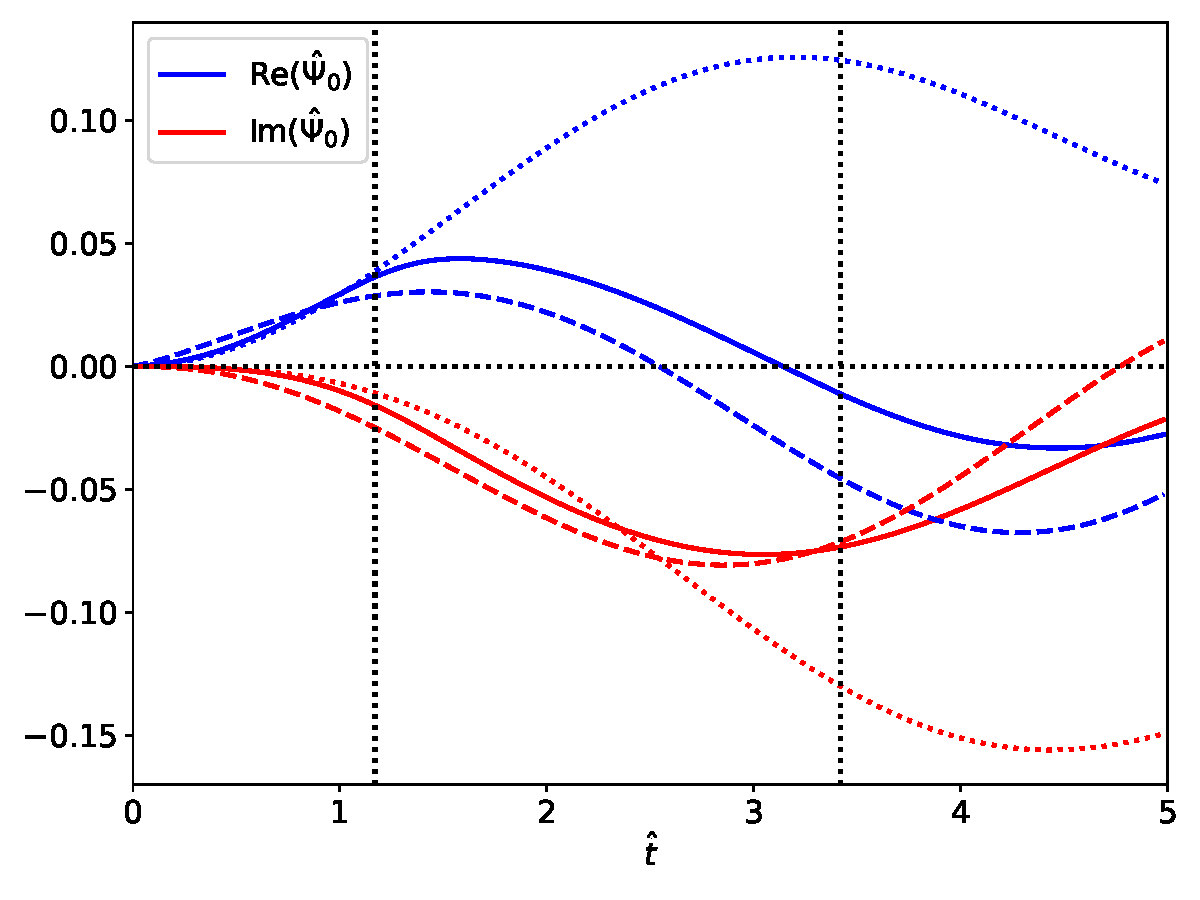
\includegraphics[width=0.8\textwidth]{Figure6.pdf}
\caption{Driven reconnected magnetic flux  at relatively early times in Reconnection Scenario 1. Here, the solid curves show the numerical solution, the dotted curves show the analytic solution in the inertial
response regime, and the dashed curves show the analytic solution in the viscous-inertial response regime. The two dotted vertical lines show the approximate
times at which the transitions from the inertial to the viscous-inertial, and from the viscous-inertial to the viscous-resistive, response regimes occur, in order from the left to the right. }\label{f6}
\end{figure}

Figure~\ref{f6} shows the driven reconnected magnetic flux at relatively early times (after the RMP is switched on) in Reconnection Scenario 1. It can be seen that, in accordance with the curve labelled 1 in Fig.~\ref{f3}, the numerical solution exactly matches
 the analytic solution in the inertial response regime at extremely early times. At intermediate times, the numerical solution deviates from the analytic solution in the inertial regime, and approximately matches
that in the viscous-inertial response regime. 

\begin{figure}[t]
\centering
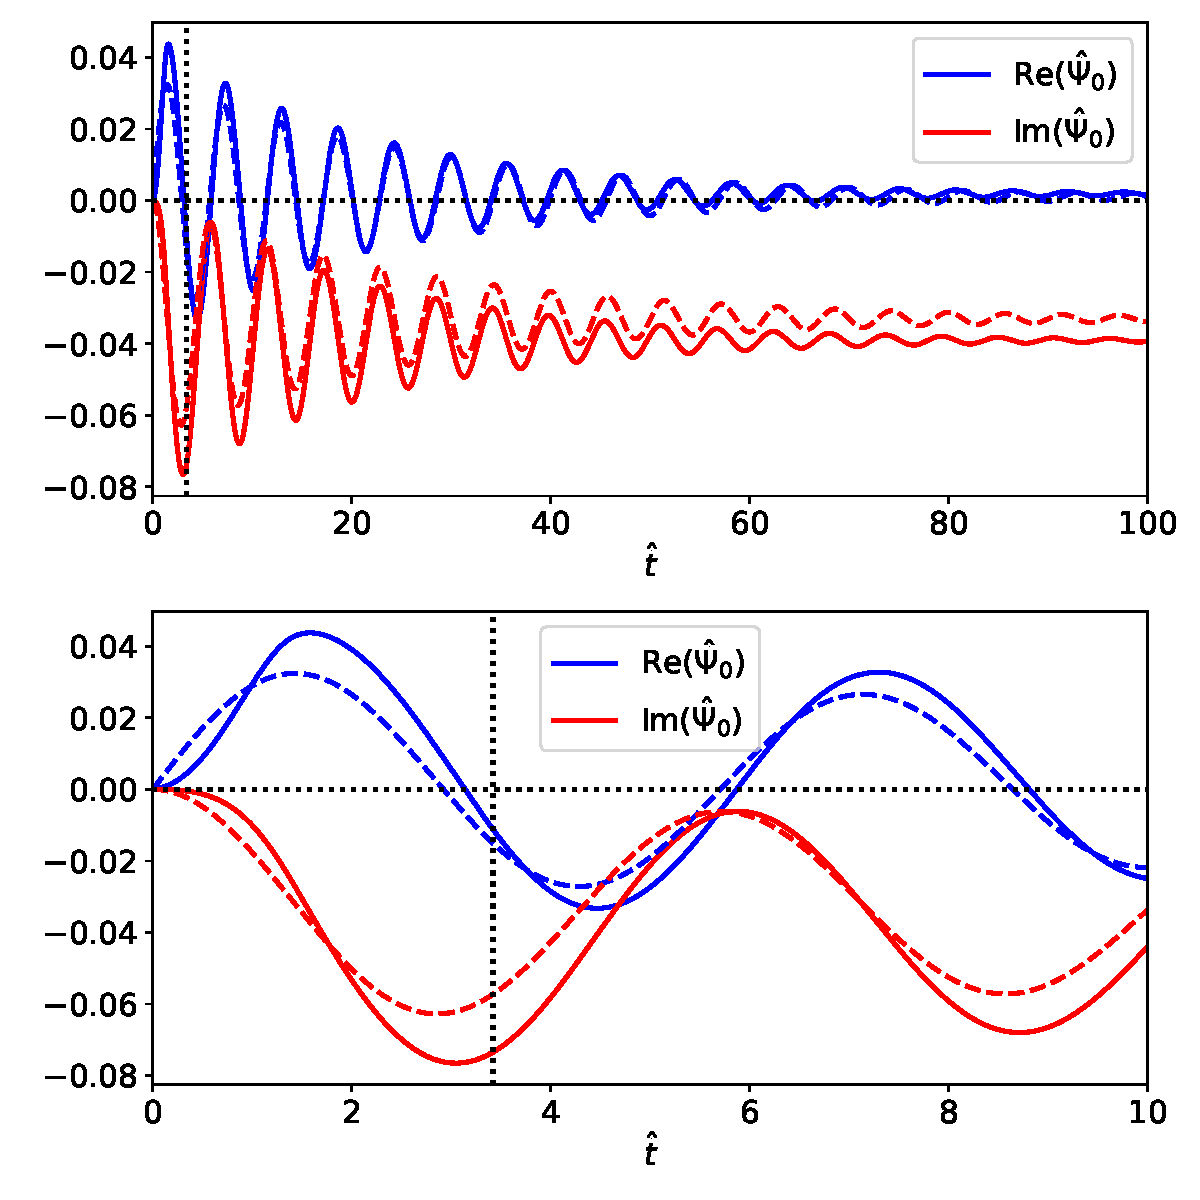
\includegraphics[width=0.8\textwidth]{Figure7.pdf}
\caption{Driven reconnected magnetic flux at relatively late times in Reconnection Scenario 1. Here, the solid curves show the numerical solution, whereas the dashed curves show the analytic solution in the 
viscous-resistive response regime. The vertical dotted line shows the approximate time at  which the transition from the viscous-inertial to the viscous-resistive response regime occurs.  }\label{f7}
\end{figure}

Figure~\ref{f7} shows the driven reconnected magnetic flux at relatively  late times in Reconnection Scenario 1. It can be seen that,  in accordance with the curve labelled 1 in Fig.~\ref{f3}, the numerical
solution matches   the analytic solution in the viscous-resistive regime fairly well at later times.  

Figures~\ref{f6} and \ref{f7} exhibit the limitations of the closed-form analytic solutions. The match with the analytic viscous-inertial solution is  approximate because the
system is only in the viscous-inertial response regime for a fairly limited period of time. Moreover, the match with the viscous-resistive solution is not perfect because the
system is not actually in the viscous-resistive response regime at $\hat{t}=0$, whereas the analytic solution assumes that this is the case. 

\begin{figure}[t]
\centering
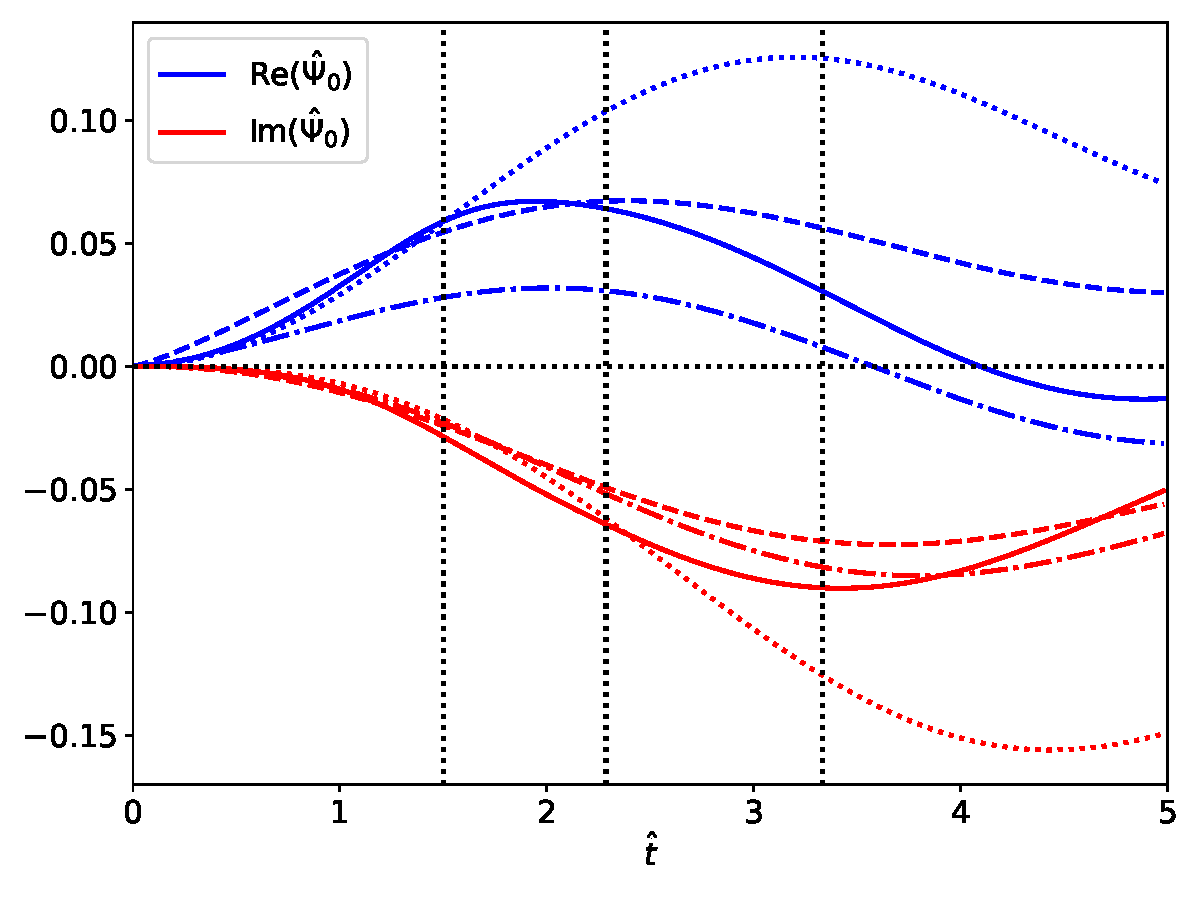
\includegraphics[width=0.8\textwidth]{Figure8.pdf}
\caption{Driven reconnected magnetic flux at relatively early times  in Reconnection Scenario 3. Here, the solid curves show the numerical solution, the dotted curves show the analytic solution in the inertial
response regime,  the dashed curves show the analytic solution in the resistive-inertial  response regime, and the dot-dashed curves show the analytic solution in the semi-collisional
regime. The three dotted vertical lines show the approximate
times at which the transitions from the inertial to the resistive-inertial, from the resistive-inertial to the semi-collisional, and from the semi-collisional to the diffusive-resistive, response regimes occur, in order from the left to the right. }\label{f8}
\end{figure}

\subsection{Reconnection Scenario 3}
Consider Reconnection Scenario 3, which is illustrated in Fig.~\ref{f3}.  The normalized layer parameters used to access this regime are listed  in Table~\ref{t1}. 

Figure~\ref{f8} shows the driven reconnected magnetic flux  at relatively early times in Reconnection Scenario 3. It can be seen that, in accordance with the curve labelled 3 in Fig.~\ref{f3}, the numerical solution 
exactly matches
 the analytic solution in the inertial response regime at extremely early times. At early intermediate times, the numerical solution deviates from the analytic solution in the inertial regime, and approximately matches
that in the resistive-inertial response regime. At late intermediate times, the numerical solution deviates from the analytic solution in the resistive-inertial regime, and approximately matches
that in the semi-collisional response regime. 

\begin{figure}[t]
\centering
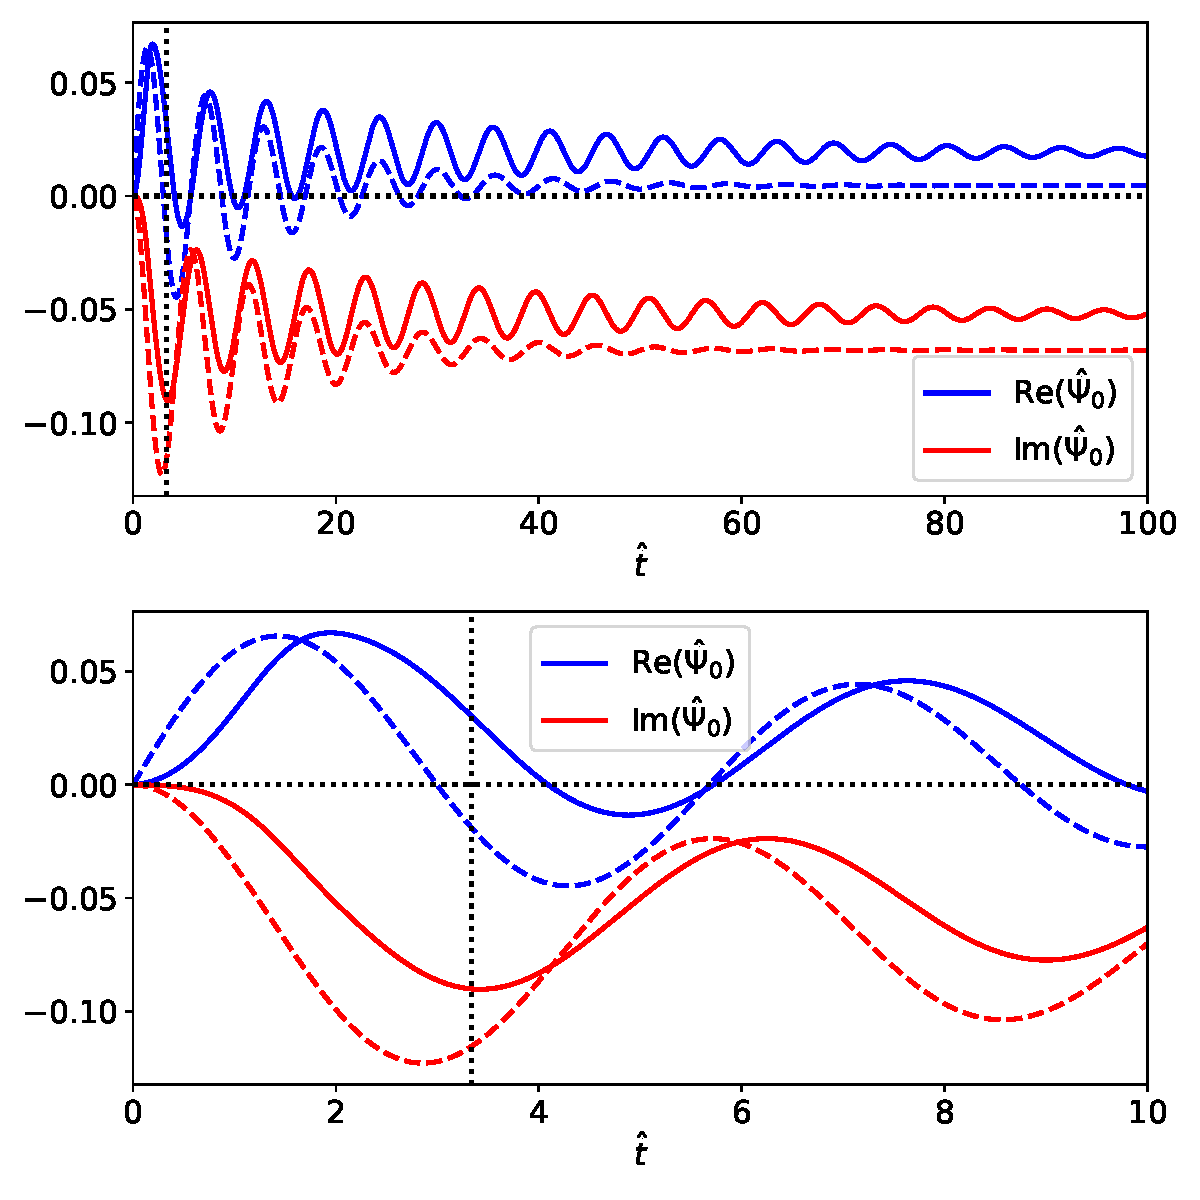
\includegraphics[width=0.8\textwidth]{Figure9.pdf}
\caption{Driven reconnected magnetic flux at relatively late times in Reconnection Scenario 3. Here, the solid curves show the numerical solution, whereas the dashed curves show the analytic solution in the 
diffusive-resistive response regime. The vertical dotted line shows the approximate time at  which the transition from the semi-collisional to the diffusive-resistive response regime occurs.  }\label{f9}
\end{figure}

Figure~\ref{f9} shows the driven reconnected magnetic flux at relatively  late times in Reconnection Scenario 3. It can be seen that,  in accordance with the curve labelled 3 in Fig.~\ref{f3}, the numerical
solution roughly matches   the analytic solution in the diffusive-resistive regime  at later times.  

Figures~\ref{f8} and \ref{f9} again illustrate the limitations of the closed-form analytic solutions. The system is not in the resistive-inertial or the semi-collisional response regimes long enough for
a good match to the respective analytic solutions to be achieved. The analytic response in the diffusive-resistive regime has the correct oscillation frequency, but the oscillations damp
away faster that those in the numerical solution. Again, one possible explanation for the mismatch  is that the numerical solution does not enter the diffusive-resistive regime until a finite time has passed since the
RMP was switched on, whereas the analytic solution assumes that the system is always in the diffusive-resistive regime. 

\begin{figure}[t]
\centering
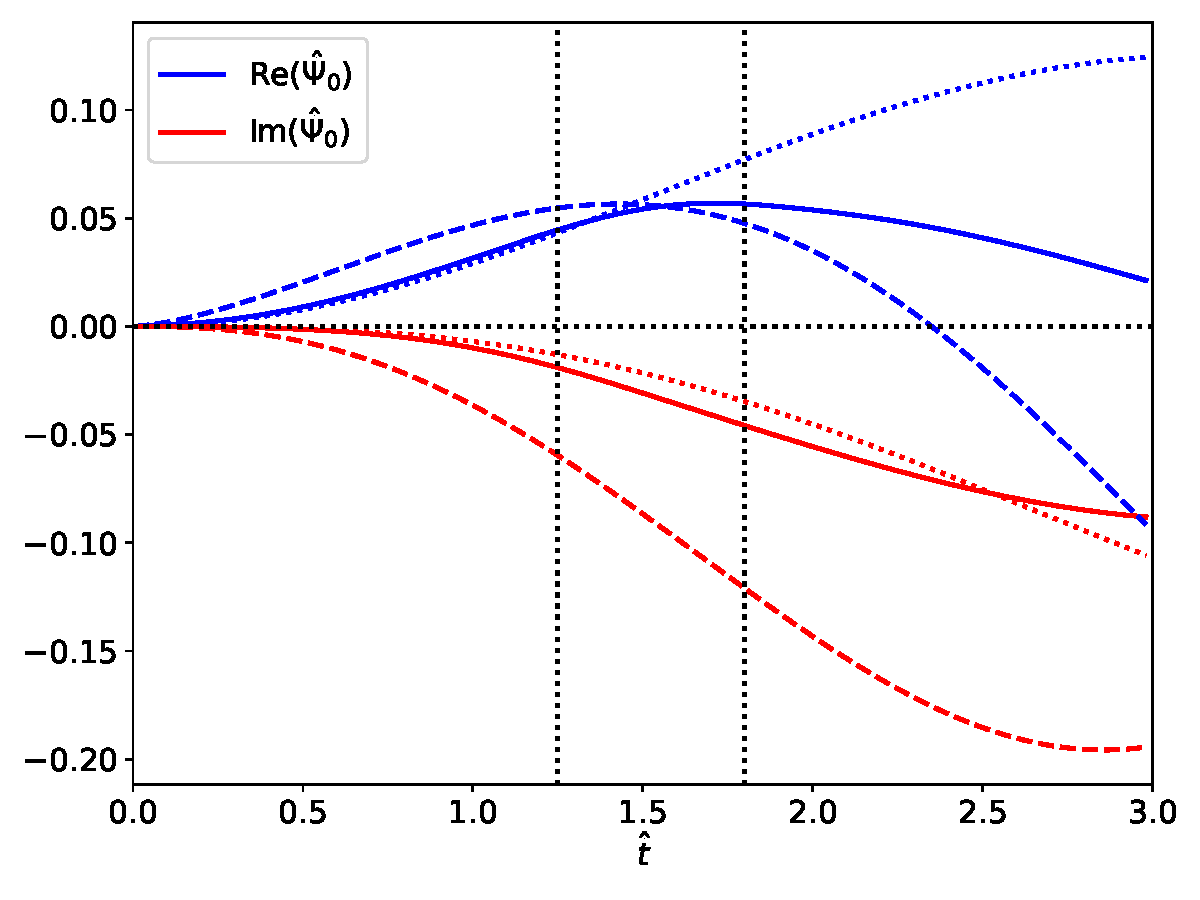
\includegraphics[width=0.8\textwidth]{Figure10.pdf}
\caption{Driven reconnected magnetic flux at relatively early times  in Reconnection Scenario 5. Here, the solid curves show the numerical solution, the dotted curves show the analytic solution in the inertial
response regime,  and the dashed curves show the analytic solution in the diffusive-inertial  response regime. The two dotted vertical lines show the approximate
times at which the transitions from the inertial to the diffusive-inertial, and from the diffusive-inertial to the diffusive-resistive,  response regimes occur, in order from the left to the right. }\label{f10}
\end{figure}

\subsection{Reconnection Scenario 5}
Consider Reconnection Scenario 5, which is illustrated in Fig.~\ref{f4}.  The normalized layer parameters used to access this regime are listed  in Table~\ref{t1}. 

Figure~\ref{f10} shows the driven reconnected magnetic flux  at relatively early times in Reconnection Scenario 5. It can be seen that, in accordance with the curve labelled 5 in Fig.~\ref{f4}, the numerical solution 
exactly matches
 the analytic solution in the inertial response regime at extremely early times. At   intermediate times, the numerical solution deviates from the analytic solution in the inertial regime toward that in the
 diffusive-inertial regime. 
 
\begin{figure}[t]
\centering
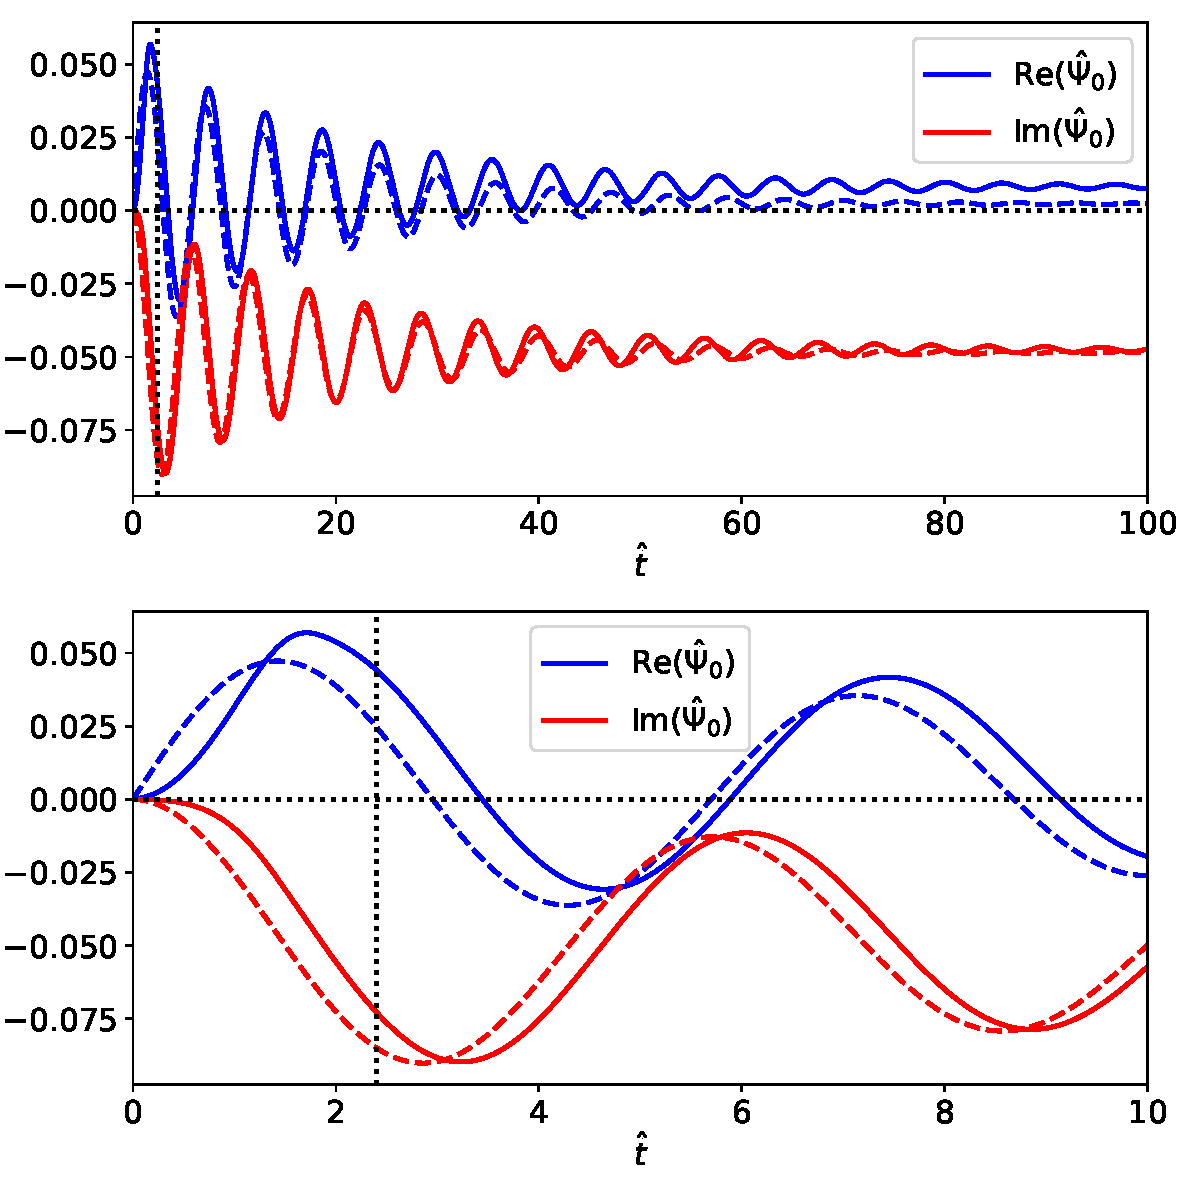
\includegraphics[width=0.8\textwidth]{Figure11.pdf}
\caption{Driven reconnected magnetic flux at relatively late times in Reconnection Scenario 5. Here, the solid curves show the numerical solution, whereas the dashed curves show the analytic solution in the 
diffusive-resistive response regime. The vertical dotted line shows the approximate time at  which the transition from the diffusive-inertial to the diffusive-resistive response regime occurs.  }\label{f11}
\end{figure}

Figure~\ref{f11} shows the driven reconnected magnetic flux at relatively  late times in Reconnection Scenario 5. It can be seen that,  in accordance with the curve labelled 5 in Fig.~\ref{f4}, the numerical
solution matches   the analytic solution in the diffusive-resistive regime fairly well at later times.  

Figures~\ref{f10} and \ref{f11} also illustrate the limitations of the closed-form analytic solutions. The system is not in the diffusive-inertial  response regimes long enough for
a good match to the analytic solution to be achieved. On the other hand, the numerical solution matches the analytic solution in the diffusive-resistive response regime
fairly well at later times. It can be seen, from a comparison between Figs.~\ref{f9} and \ref{f11}, that a better match to the analytic diffusive-resistive solution is achieved in this case because the numerical
solution is a better match to the analytic solution on entry into the diffusive-resistive regime. 

\section{Summary and Discussion}
This paper employs asymptotic matching techniques to investigate the drift-MHD response of a flowing tokamak plasma to a static RMP that is switched on suddenly in time.

The resonant layer in the immediate vicinity of the rational surface is analyzed by means of a Fourier-Laplace transform. The layer is characterized by three quantities:
the conventional layer response index, $\hat{\mit\Delta}_s$, the ratio of the magnetic flux at the edge of the layer to that at the center, $F_s$, and the normalized layer thickness, $\hat{\delta}$. 
Seven different resonant plasma response regimes are identified. 
These are the inertial, the viscous-inertial, the diffusive-inertial, the resistive-inertial, the semi-collisional, the
viscous-resistive, and the diffusive-resistive regimes. See Figs.~\ref{f1} and \ref{f2}. Expressions for $\hat{\mit\Delta}_s$, $F_s$, and $\hat{\delta}$ in each regime are derived. See Sects.~\ref{inertial}--\ref{diffusive}. 

The driven reconnected magnetic
flux at the rational surface can be expressed as a contour integral in the space of the complex Laplace transform variable conjugate to time. See Eq.~(\ref{e29}). 
In each resonant response regime, it is possible to perform the integral to obtain a closed-form analytic expression for the driven magnetic flux as a function of time. See~Eqs.~(\ref{inertialp}),
(\ref{vip}), (\ref{dip}), (\ref{rip}), (\ref{scpx}), (\ref{vrp}), and (\ref{drp}). The small and large time limits of each expression are obtained. See Eqs.~(\ref{inertials}), (\ref{vis}), (\ref{dis}), (\ref{ris}), (\ref{scs}), 
(\ref{vrs}), and (\ref{drs}), 
as well as (\ref{inertiall}), (\ref{vil}), (\ref{dil}), (\ref{ril}), (\ref{scl}), (\ref{vrl}), and (\ref{drl}). 

Depending on the values of the normalized parameters that govern the resonant layer, seven different reconnection scenarios are identified that describe how the
driven reconnected magnetic flux at the rational surface evolves though the various different resonant response regimes as a function of time. See Sect.~\ref{scenarios}, and Figs.~\ref{f3} and \ref{f4}. 

The driven reconnected magnetic flux at the rational surface is be calculated as a function of time  by two alternative  methods.  The first solution  method, which is exact,  involves numerically 
evaluating the aforementioned contour integral. The second solution method, which is only approximate,  but much less time consuming,  involves evaluating the closed-form analytic expressions. The results of the two
solution methods are compared in three different reconnection scenarios that involve all seven resonant response regimes. In all cases, at very early times, the driven magnetic flux exactly matches that
predicted by the inertial regime analytic solution. The agreement between the numerical solution and the intermediate-time analytic response regimes  is only approximate because the
system does not spend a sufficient amount of time in these regimes for an exact match to be achieved. The agreement between the numerical solution and the late-time, constant-$\psi$,
analytic response regimes is better, but is not exact because the analytic solutions assume that the system is always in the late-time regime, whereas, in reality, the
system is in other regimes at early and intermediate times. 

\section*{Funding}
This research was supported by the U.S.\ Department of Energy, Office of Science, Office of Fusion Energy Sciences, under  contract DE-FG02-04ER54742. 

\section*{Data Availability Statement}
The data that support the findings of this study are available from the corresponding author upon reasonable request.

\appendix

\section{Outer Region}\label{outer}
\subsection{Introduction}
Consider the cylindrical plasma equilibrium introduced in Sect.~\ref{s2a}. Suppose that the plasma is subject to an RMP with $m$ periods in the
poloidal direction, and $n$ periods in the toroidal direction. The perturbation is resonant at the rational surface, radius $r_s$, at which $q(r_s)=m/n$. 
This appendix considers the response of the plasma to the RMP in the outer region: that is, everywhere apart from the immediate vicinity of the rational surface. 

\subsection{Cylindrical Tearing Mode Equation}
In the outer region, the perturbed magnetic field can be written $\delta {\bf B} = r_s\,B_\varphi\,\nabla\delta \psi\times{\bf e}_z$, where
\begin{equation}\label{e2}
\delta\psi(r,\zeta,t) = \psi_1(r,t)\,{\rm e}^{\,{\rm i}\,\zeta},
\end{equation}
and $\zeta=m\,\theta-n\,\varphi$ is a helical angle.\cite{err1}

The function $\psi_1(r,t)$ satisfies the {\em cylindrical tearing mode equation},\cite{err1,ric3,cyl,wes}
\begin{equation}\label{e111}
\frac{\partial^2\psi_1}{\partial\hat{r}^{\,2}} + \frac{1}{\hat{r}}\,\frac{\partial\psi_1}{\partial\hat{r}}-\frac{m^2}{\hat{r}^{\,2}}\,\psi_1
- \frac{J_\varphi'\,\psi_1}{\hat{r}\,(1/q-n/m)} = 0,
\end{equation}
where $\hat{r}=r/a$, $J_\varphi'(\hat{r})= dJ_\varphi/d\hat{r}$,
\begin{align}
J_\varphi(\hat{r}) &= \frac{R_0\,\mu_0\,j_\varphi}{B_\varphi}.
\end{align}
Let us assume that $J_\varphi(\hat{r})$ is a continuous function, and that $J_\varphi(\hat{r}>1)=0$.  (In other words, the region $\hat{r}>1$ is assumed to be a vacuum.)
Note that Eq.~(\ref{e111}) is singular at the  rational surface. The singularity is indicative of the breakdown of the equations of linearized, 
marginally-stable, ideal-MHD in the  inner region.
 
\subsection{Solution of Cylindrical Tearing Mode Equation}\label{scly}
Suppose that the plasma is surrounded by a rigid conducting wall located at $r=b$, where $b>a$. 
Let $\psi_1(b,t) = {\mit\Psi}_b(t)$, where ${\mit\Psi}_b(t)$ is a complex dimensionless quantity that specifies the amplitude and phase of the
RMP to which the plasma is subject. The most general solution to the cylindrical tearing mode equation in the outer region is written 
\begin{equation}\label{e73}
\psi_1(\hat{r},t) = {\mit\Psi}_s(t)\,\hat\psi_s(\hat{r}) + {\mit\Psi}_b(t)\,\hat{\psi}_b(\hat{r}), 
\end{equation}
Here, $\hat{\psi}_s(\hat{r})$ is a real continuous solution of Eq.~(\ref{e111}) that satisfies 
\begin{align}
\hat{\psi}_s(0) &= 0,\label{e11a}\\[0.5ex]
\hat{\psi}_s(\hat{r}_s)&= 1,\label{e12a}\\[0.5ex]
\hat{\psi}_s(\hat{r}\geq \hat{b}) &= 0,\label{e13a}
\end{align}
where $\hat{r}_s=r_s/a$, and $\hat{b}= b/a$. 
Moreover, $\hat{\psi}_b(\hat{r})$ is a real continuous solution of Eq.~(\ref{e111}) that satisfies
\begin{align}
\hat{\psi}_b(\hat{r}\leq \hat{r}_s) &= 0,\\[0.5ex]
\hat{\psi}_b(\hat{b})&= 1.\label{e109}
\end{align}
Note that the dimensionless complex quantity ${\mit\Psi}_s(t)$ parameterizes the amplitude and phase  of the
helical magnetic flux driven  by the RMP at the interface between the inner and the outer regions.

\subsection{Calculation of $\hat{\psi}_s(\hat{r})$}\label{psis}
In the limit $0<\hat{r}\ll 1$, the solution of Eq.~(\ref{e111}), subject to the boundary condition (\ref{e11a}), is 
\begin{equation}\label{e81}
\hat{\psi}_s(\hat{r})\propto \hat{r}^{\,m} + \kappa_0\,\hat{r}^{\,m+2},
\end{equation}
where 
\begin{equation}
\kappa_0 = - \frac{x_0}{4\,(m+1)\,(1/q_0-n/m)},
\end{equation}
 and $q_0=q(0)$, with $x_0=\lim_{\hat{r}\rightarrow 0}(-J_\varphi'/\hat{r})$. 

Let $\hat{x} = (\hat{r}-\hat{r}_s)/\hat{r}_s$. 
In the immediate vicinity of the rational surface, the continuous solution to Eq.~(\ref{e111}), subject to the constraint 
(\ref{e12a}), is 
\begin{equation}\label{e18}
\hat{\psi}_s(\hat{x}) = 1+{\mit\Delta}_{s+}\,\hat{x} +\alpha_s\,\hat{x}\,\ln|\hat{x}| + {\cal O}(\hat{x}^2)
\end{equation}
for $\hat{x}>0$, and 
\begin{equation}\label{e19}
\hat{\psi}_s(\hat{x}) = 1+{\mit\Delta}_{s-}\,\hat{x} +\alpha_s\,\hat{x}\,\ln|\hat{x}| + {\cal O}(\hat{x}^2)
\end{equation}
for $\hat{x}<0$, where
\begin{equation}
\alpha_s = -\left(\frac{\hat{r}\,q\,J_\varphi'}{s}\right)_{\hat{r}=\hat{r}_s},
\end{equation}
and $s=d\ln q/d\ln r$ is the {\em magnetic shear}. 
In particular,
\begin{equation}\label{e86}
{\mit\Delta}_{s\,\pm} = \frac{\hat{r}}{\hat{\psi_s}}\,\frac{d\hat{\psi}_s}{d\hat{r}}-\alpha_s\,(1+\ln |\hat{x}|),
\end{equation}
in the limit that $\hat{x}\rightarrow 0_{\pm}$.

Finally, solving Eq.~(\ref{e111}) outside the plasma (where $J_\varphi'=0$), subject to the boundary condition (\ref{e13a}), yields 
\begin{equation}\label{e87}
\left(\frac{\hat{r}}{\hat{\psi}_s}\,\frac{d\hat{\psi}_s}{d\hat{r}}\right)_{\hat{r}=1} = -m\left(\frac{\hat{b}^{\,2m}+1}{\hat{b}^{\,2m}-1}\right).
\end{equation}

We can calculate $\hat{\psi}_s(\hat{r})$ by, first, launching a solution of Eq.~(\ref{e111}) from the magnetic
axis, subject to the boundary condition (\ref{e81}), and integrating to just inside the rational surface.
Next, we launch a second solution of  Eq.~(\ref{e111}) from  the plasma boundary, subject to the boundary condition (\ref{e87}),   and integrate to just outside the rational surface. The two solutions are then rescaled subject to the
constraint $\hat{\psi}_s(\hat{r}_s)=1$. The real dimensionless quantity
\begin{align}\label{e88}
E_{ss} &\equiv \left[\hat{r}\,\frac{d\hat{\psi}_s}{d\hat{r}}\right]^{\hat{r}=\hat{r}_{s+}}_{\hat{r}=\hat{r}_{s-}} ={\mit\Delta}_{s+} -{\mit\Delta}_{s-}
\end{align}
is the  conventional tearing stability index.\cite{fkr} It is assumed that $E_{ss}<0$, which implies that the $m/n$ tearing mode is intrinsically stable. Thus, any reconnected magnetic flux that develops at the rational surface is
due solely to the action of the RMP to which the plasma is subject.

\subsection{Calculation of $\hat{\psi}_b(\hat{r})$}\label{psib}
In order to calculate $\hat{\psi}_b(\hat{r})$, we launch a solution of Eq.~(\ref{e111}) from just outside the
rational surface, such that 
\begin{align}
\hat{\psi}_b(\hat{r}_s) &= 0,\\[0.5ex]
\frac{d\hat{\psi}_b(\hat{r}_s)}{d\hat{r}} &= \frac{1}{\hat{r}_s},
\end{align}
and then integrate it to  the plasma boundary. 
Let
\begin{align}
\alpha_b &= \frac{1}{2m}\left[m\,\hat{b}^{\,m}\,\hat{\psi}_b(1)+ \hat{b}^{\,m}  \,\frac{d\hat{\psi}_b(1)}{d\hat{r}}\right],\\[0.5ex]
\beta_b &= \frac{1}{2m}\left[m\,\hat{b}^{-m}\,\hat{\psi}_b(1)- \hat{b}^{-m}\,\frac{d\hat{\psi}_b(1)}{d\hat{r}}\right],\\[0.5ex]
\gamma_b&= \alpha_b+\beta_b.
\end{align}
The boundary condition (\ref{e109}) is satisfied by dividing our solution by $\gamma_b$. 
Let us define the real dimensionless quantity 
\begin{equation}\label{e93}
E_{sb} \equiv \left[\hat{r}\,\frac{d\hat{\psi}_b}{d\hat{r}}\right]_{\hat{r}=\hat{r}_{s+}} = \frac{1}{\gamma_b},
\end{equation}
which parameterizes the coupling between the wall and the rational surface. 

\subsection{Asymptotic Matching}
The complex dimensionless quantity 
\begin{align}\label{e30}
{\mit\Delta\Psi}_{s}(t) &= \left[\hat{r}\,\frac{\partial\psi_1}{\partial\hat{r}}\right]_{\hat{r}=\hat{r}_{s-}}^{\hat{r}=\hat{r}_{s+}}
\end{align}
parameterizes the amplitude and phase of the helical current sheet that is induced in the inner region. 
Asymptotic matching between the inner and the outer regions yields
\begin{align}\label{e31a}
{\mit\Delta\Psi}_{s}(t) &= E_{ss}\,{\mit\Psi}_s(t)+E_{sb}\,{\mit\Psi}_b(t),
\end{align}
where use has been made of Eqs.~(\ref{e73}), (\ref{e88}), (\ref{e93}), and (\ref{e30}). 

\section{Inner Region}\label{inner}
\subsection{Introduction}
The inner region, which lies in the immediate vicinity of the rational surface, is assumed to be governed by the  four-field drift-MHD model described in Ref.~\onlinecite{err3}. This
model is an extension of a model introduced in Ref.~\onlinecite{err2}, and is ultimately based on the four-field model of Ref.~\onlinecite{hkm}. 

\subsection{Useful Definitions}
The plasma is assumed to consist of two species. First, electrons of mass $m_e$, electrical charge $-e$, 
number density $n_e$, and temperature $T_e$.  Second, ions of mass $m_i$, electrical charge $+e$,  
number density $n_e$, and temperature $T_i$. Let $p=n_e\,(T_e+T_i)$ be the total plasma pressure. 

It is helpful to define $n_0 = n_e(r_s)$, $p_0= p(r_s)$,
\begin{align}
\eta_e &=\left.\frac{d\ln T_e}{d\ln n_e}\right|_{r=r_s},\label{e211}\\[0.5ex]
\eta_i &= \left.\frac{d\ln T_i}{d\ln n_e}\right|_{r=r_s},\\[0.5ex]
\iota &\equiv \left(\frac{dp_e}{dp_i}\right)_{r_s}= \left(\frac{T_e}{T_i}\right)_{r=r_s}\left(\frac{1+\eta_e}{1+\eta_i}\right),\label{e213}
\end{align}
where $n_e(r)$, $p(r)$, $p_e(r)= n_e(r)\,T_e(r)$, $p_i(r)= n_e(r)\,T_i(r)$, $T_e(r)$, and $T_i(r)$ refer to
density, total pressure, electron pressure, ion pressure,  electron temperature, and ion temperature profiles, respectively, in the absence of the RMP. 

For the sake of simplicity, the perturbed electron and ion temperature profiles are assumed to be functions of
the perturbed electron number density profile in the immediate vicinity of the rational surface. In other words, $T_e=T_e(n_e)$ and $T_i=T_i(n_e)$. This
implies that $p=p(n_e)$. 
The  MHD velocity, which is the velocity of a
fictional MHD fluid,\cite{haz1} is defined as ${\bf V}={\bf V}_E + V_{\parallel\,i}\,{\bf b}$, where ${\bf V}_E$ is the
${\bf E}\times {\bf B}$ drift velocity, $V_{\parallel\,i}$  the parallel component of the ion fluid
velocity, ${\bf b}= {\bf B}/|{\bf B}|$, and ${\bf B}$ the magnetic field-strength. 

\subsection{Dimensionless Fields}
The four  dimensionless fields in our four-field model---namely, $\psi$, $\phi$, $N$, and $V$---have the following
definitions:
\begin{align}\label{e10}
\nabla\psi &= \frac{{\bf e}_\parallel\times{\bf B}} {r_s\,B_\varphi},\\[0.5ex]
\nabla\phi &= \frac{{\bf e}_\parallel\times {\bf V}}{r_s\,V_A},\label{e40a}\\[0.5ex]
N &=-\hat{d}_i\left(\frac{p-p_0}{B_\varphi^{\,2}/\mu_0}\right),\\[0.5ex]
V &= \hat{d}_i\left(\frac{{\bf e}_\parallel\cdot {\bf V}}{V_A}\right).\label{e13}
\end{align}
Here,   ${\bf e}_\parallel = (0,\,\epsilon/q_s,\,1)$, $\epsilon = r/R_0$, $q_s=m/n$, 
$V_A =(B_\varphi/\sqrt{\mu_0\,n_0\,m_i})_{r_s}$ is the Alfv\'{e}n speed, 
$d_i = \sqrt{m_i/(n_0\,e^{\,2}\,\mu_0)_{r_s}}$ the collisionless ion skin-depth,
and $\hat{d}_i=d_i/r_s$. 
 Our
model also employs the auxiliary dimensionless  field
\begin{align}\label{e16}
J=-\frac{2\,\epsilon_s}{q_s}+\hat{\nabla}^2\psi,
\end{align}
where 
$\epsilon_s=r_s/R_0$, and $\hat{\nabla} = r_s\,\nabla$. Note that 
\begin{equation}\label{e44}
\psi(r,\zeta,t) = \psi_0(r)+ \psi_1(r,t)\,{\rm e}^{\,{\rm i}\,\zeta},
\end{equation}
where
\begin{equation}\label{e45}
\psi_0(r) = \frac{1}{R_0\,r_s}\int_{r_s}^r r'\left[\frac{n}{m}-\frac{1}{q(r')}\right]dr'.
\end{equation}

\subsection{Four-Field Model}
Our four-field model takes the form:\cite{fw,err2,err3}
\begin{align}
\frac{\partial\psi}{\partial\hat{t}}&= [\phi,\psi] -\iota_e\,[N,\psi]
+\hat{\eta}_\parallel\,J + \hat{E}_\parallel,\label{e16a}\\[0.5ex]
\frac{\partial \hat{\nabla}^2\phi}{\partial \hat{t}}&= [\phi,\hat{\nabla}^2\phi] - \frac{\iota_i}{2}\left(\hat{\nabla}^2[\phi,N] + [\hat{\nabla}^2\phi,N] + [\hat{\nabla}^2 N,\phi]\right) + [J,\psi] \nonumber\\[0.5ex]&\phantom{=}+\hat{\chi}_\varphi  \,\hat{\nabla}^4\!\left(\phi + \iota_i\,N\right), \\[0.5ex]
\frac{\partial N}{\partial \hat{t}}&= [\phi,N] +c_\beta^{\,2}\,[V,\psi] +\hat{d}_\beta^{\,2}\,[J,\psi]
+ \hat{\chi}_\perp\,\hat{\nabla}^{\,2}N,\label{e48}\\[0.5ex]
\frac{\partial V}{\partial\hat{t}}&= [\phi,V] +[N,\psi] + \hat{\chi}_\varphi\,\hat{\nabla}^2 V.\label{e21}
\end{align}
Here, $[A,B]\equiv \hat{\nabla} A\times \hat{\nabla} B\cdot {\bf e}_\parallel$, $\iota_e=\iota/(1+\iota)$, $\iota_i=1/(1+\iota)$, $\hat{t} = t/(r_s/V_A)$, $\hat{\eta}_{\parallel} = \eta_{\parallel}/(\mu_0\,r_s\,V_A)$, $\hat{E}_\parallel = E_\parallel/(B_\varphi\,V_A)$, 
$\hat{\chi}_\varphi= \chi_\varphi/(r_s\,V_A)$, $\hat{\chi}_\perp=\chi_\perp/(r_s\,V_A)$, where $\eta_{\parallel}$ is the parallel  plasma electrical
resistivity at the rational surface, $E_\parallel$ the parallel inductive electric field that maintains the equilibrium toroidal
plasma current in the vicinity of the rational surface,  $\chi_\varphi$  the anomalous perpendicular ion momentum
diffusivity at the rational surface, and $\chi_\perp$ the anomalous perpendicular energy diffusivity at the rational surface.
Moreover, $d_\beta=c_\beta\,d_i$, and $\hat{d}_\beta=d_\beta/r_s$, where $c_\beta = \sqrt{\beta/(1+\beta)}$, and
$\beta=(5/3)\,\mu_0\,p_0/B_\varphi^{\,2}$. Here, $d_\beta$ is usually referred to as the ion sound-radius. 
Note that we have neglected parallel energy transport in Eq.~(\ref{e48}) because we expect the radial width of the inner region to be less than the critical width above which parallel transport forces the temperature and density profiles to be magnetic flux-surface functions.\cite{hel}

\subsection{Matching to Plasma Equilibrium}
The unperturbed plasma equilibrium is such that
${\bf B} = (0,\,B_\theta(r),\,B_\varphi)$,  $p = p(r)$,
${\bf V} = (0,\,V_E(r),\,V_\varphi(r))$,
where 
$V_E(r)\simeq -E_r/B_\varphi$
 is the (dominant $\theta$-component of the) ${\bf E}\times {\bf B}$ drift velocity. Now, the inner region is assumed to have a radial thickness that is
much smaller than $r_s$.   Hence, we only need to evaluate plasma equilibrium quantities in the immediate vicinity of the rational
surface. Equations~(\ref{e10})--(\ref{e13}) and (\ref{e44})--(\ref{e45}) suggest that 
\begin{align}
\psi(\hat{x})&= \frac{\hat{x}^{\,2}}{2\,\hat{L}_s},\label{e23}\\[0.5ex]
\phi(\hat{x}) &= - \hat{V}_E\,\hat{x},\\[0.5ex]
N(\hat{x}) &= -\hat{V}_\ast\,\hat{x},\\[0.5ex]
V &= \hat{V}_\parallel,\label{e26}
\end{align}
where $\hat{x}= (r-r_s)/r_s$, 
 $\hat{L}_s=L_s/r_s$,  $L_s=R_0\,q_s/s_s$, 
  $\hat{V}_E= V_E(r_s)/V_A$,
$\hat{V}_\ast= V_\ast(r_s)/V_A$,
$V_\ast(r) = (dp/dr)/(e\,n_0\,B_\varphi)$ 
is the (dominant $\theta$-component of the) diamagnetic velocity,
  and 
 $\hat{V}_\parallel=\hat{d}_i\, V_\varphi(r_s)/V_A$. Here, $s_s=s(r_s)$. We also deduce that 
 \begin{align}\label{e28}
 J (\hat{x})&= -\left(\frac{2}{s_s}-1\right)\frac{1}{\hat{L}_s},
\end{align} 
and $ \hat{E}_\parallel(\hat{x}) =(2/s_s-1) (\hat{\eta}_\parallel/\hat{L}_s)$.

\subsection{Linearized Layer Equations}
In accordance with Eqs.~(\ref{e16}), (\ref{e44}), and (\ref{e23})--(\ref{e28}), let us write
\begin{align}\label{e31}
\psi(\hat{x},\zeta,\hat{t}) &= \frac{\hat{x}^{\,2} }{2\,\hat{L}_s}+ \tilde{\psi}(\hat{x},\hat{t})\,{\rm e}^{\,{\rm i}\,\zeta},\\[0.5ex]
\phi(\hat{x},\zeta,\hat{t}) &=-\hat{V}_E\,\hat{x}+ \tilde{\phi}(\hat{x},\hat{t})\,{\rm e}^{\,{\rm i}\,\zeta},\\[0.5ex]
N(\hat{x},\zeta,\hat{t}) &= -\hat{V}_\ast\,\hat{x}+\iota_e\,\tilde{N}(\hat{x},\hat{t})\,{\rm e}^{\,{\rm i}\,\zeta},\\[0.5ex]
V(\hat{x},\zeta,\hat{t}) &= \hat{V}_\parallel +\iota_e\,\tilde{V}(\hat{x},\hat{t})\,{\rm e}^{\,{\rm i}\,\zeta},\\[0.5ex]
J(\hat{x},\zeta,\hat{t}) &=-\left(\frac{2}{s_s}-1\right)\!\frac{1}{\hat{L}_s}+ \hat{\nabla}^2\tilde{\psi}(\hat{x},\hat{t})\,{\rm e}^{\,{\rm i}\,\zeta}.\label{e36}
\end{align}
Substituting Eqs.~(\ref{e31})--(\ref{e36}) into Eqs.~(\ref{e16a})--(\ref{e21}), 
 and only retaining terms that
are first order in perturbed quantities, we obtain the following set of linearized layer equations:
\begin{align}\label{e37}
\tau_H\,\frac{\partial\tilde{\psi}}{\partial t}-{\rm i}\,n\,(\omega_E +\omega_{\ast\,e})\,\tau_H\,\tilde{\psi} &= -{\rm i} \,\hat{x}\,(\tilde{\phi}-\tilde{N})+ S^{-1}\,\hat{\nabla}^2\tilde{\psi},\\[0.5ex]
\tau_H\,\frac{\partial\hat{\nabla}^2\tilde{\phi}}{\partial t}-{\rm i}\,n\,(\omega_E+\omega_{\ast\,i})\,\tau_H\,\hat{\nabla}^2\tilde{\phi} &= -{\rm i}\,\hat{x}\,\hat{\nabla}^2\tilde{\psi}+S^{-1}\,P_\varphi\,\hat{\nabla}^4\!\left(\tilde{\phi} + \frac{\tilde{N}}{\iota}\right),\\[0.5ex]
\tau_H\,\frac{\partial\tilde{N}}{\partial t}-{\rm i}\,n\,\omega_E\,\tau_H\,\tilde{N} &= {\rm i}\,n\,\omega_{\ast\,e}\,\tau_H\,\tilde{\phi}-{\rm i}\,c_\beta^{\,2}\,\hat{x}\,\tilde{V} - {\rm i}\,\iota_e\,\hat{d}_\beta^{\,2}\,\hat{x}\,\hat{\nabla}^2\tilde{\psi}\nonumber\\[0.5ex]
&\phantom{=} + S^{-1}\,P_\perp\,\hat{\nabla}^2 \tilde{N},\label{e60}\\[0.5ex]
\tau_H\,\frac{\partial\tilde{V}}{\partial t}-{\rm i}\,n\,\omega_E\,\tau_H\,\tilde{V} &= -{\rm i}\,n\,\omega_{\ast\,e}\,\tau_H\,\tilde{\psi} - {\rm i}\,\hat{x}\,\tilde{N}
+ S^{-1}\,P_\varphi\,\hat{\nabla}^2\tilde{V}.\label{e40}
\end{align}
Here, 
$\tau_H = L_s/(m\,V_A)$ 
is the  hydromagnetic time, 
$\omega_E =-(q_s/r_s)\,V_E(r_s)=- (d{\mit\Phi}/{d\psi_p})_{r_s}$
  the 
${\bf E}\times {\bf B}$ frequency, 
$\omega_{\ast\,e} = \iota_e\,(q_s/r_s)\,V_\ast(r_s) = [(dp_e/d\psi_p)/(e\,n_e)]_{r_s}$
the electron diamagnetic requency,
$\omega_{\ast\,i} =-\iota_i\,(q_s/r_s)\,V_\ast(r_s)=- [(dp_i/d\psi_p)/(e\,n_e)]_{r_s}$
 the   ion diamagnetic frequency,  ${\mit\Phi}(r)$ the equilibrium electrostatic potential, $\psi_p(r)= B_\varphi\int_0^r dr'\,r'/q(r')$ the equilibrium poloidal magnetic flux, 
$S=\tau_R/\tau_H$
 the   Lundquist number, 
$\tau_R =( \mu_0\,r_s^{\,2}/\eta_\parallel)_{r_s}$
 the resistive diffusion time, 
$\tau_\varphi
= (r^2/\chi_\varphi)_{r_s}$
the  toroidal momentum confinement time, and 
$\tau_\perp = (r^2/\chi_\perp)_{r_s}$ the energy confinement time.
  Furthermore, $P_\varphi = \tau_R/\tau_\varphi$ and $P_\perp = \tau_R/\tau_\perp$ are  magnetic Prandtl numbers. 
  Note that $\iota=-\omega_{\ast\,e}/\omega_{\ast\,i}$. 

In the following, in accordance with the analysis of Refs.~\onlinecite{err2} and \onlinecite{err3}, we shall
neglect the term  $-{\rm i}\,c_\beta^{\,2}\,\hat{x}\,\tilde{V}$ in Eq.~(\ref{e60}). This approximation is only valid in low-$\beta$ plasmas, and 
 is equivalent to  the neglect of ion parallel dynamics in the inner region. The low-$\beta$ approximation effectively converts our four-field model into the following three-field model:
\begin{align}\label{e64}
\tau_H\,\frac{\partial\tilde{\psi}}{\partial t}-{\rm i}\,n\,(\omega_E +\omega_{\ast\,e})\,\tau_H\,\tilde{\psi} &= -{\rm i} \,\hat{x}\,(\tilde{\phi}-\tilde{N})+ S^{-1}\,\hat{\nabla}^2\tilde{\psi},\\[0.5ex]
\tau_H\,\frac{\partial\hat{\nabla}^2\tilde{\phi}}{\partial t}-{\rm i}\,n\,(\omega_E+\omega_{\ast\,i})\,\tau_H\,\hat{\nabla}^2\tilde{\phi} &= -{\rm i}\,\hat{x}\,\hat{\nabla}^2\tilde{\psi}+S^{-1}\,P_\varphi\,\hat{\nabla}^4\!\left(\tilde{\phi} + \frac{\tilde{N}}{\iota}\right),\\[0.5ex]
\tau_H\,\frac{\partial\tilde{N}}{\partial t}-{\rm i}\,n\,\omega_E\,\tau_H\,\tilde{N} &={\rm i}\,n\,\omega_{\ast\,e}\,\tau_H\,\tilde{\phi} - {\rm i}\,\iota_e\,\hat{d}_\beta^{\,2}\,\hat{x}\,\hat{\nabla}^2\tilde{\psi}+ S^{-1}\,P_\perp\,\hat{\nabla}^2 \tilde{N}.\label{e66}
\end{align}

\subsection{Laplace Transformed Layer Equations}
Let us Laplace transform Eqs.~(\ref{e64})--(\ref{e66}) by operating on them with
$\int_0^\infty (\cdots)\,{\rm e}^{-g\,t}\,dt$. Assuming that all fields are zero at $t=0$, we obtain
\begin{align}\label{e67}
g\,\tau_H\,\bar{\psi}-{\rm i}\,n\,(\omega_E +\omega_{\ast\,e})\,\tau_H\,\bar{\psi} &= -{\rm i} \,\hat{x}\,(\bar{\phi}-\bar{N})+ S^{-1}\,\hat{\nabla}^2\bar{\psi},\\[0.5ex]
g\,\tau_H\,\hat{\nabla}^2\bar{\phi}-{\rm i}\,n\,(\omega_E+\omega_{\ast\,i})\,\tau_H\,\hat{\nabla}^2\,\bar{\phi} &= -{\rm i}\,\hat{x}\,\hat{\nabla}^2\bar{\psi}+S^{-1}\,P_\varphi\,\hat{\nabla}^4\!\left(\bar{\phi} + \frac{\bar{N}}{\iota}\right),\\[0.5ex]
g\,\tau_H\,\bar{N}-{\rm i}\,n\,\omega_E\,\tau_H\,\bar{N} &= {\rm i}\,n\,\omega_{\ast\,e}\,\tau_H\,\bar{\phi} - {\rm i}\,\iota_e\,\hat{d}_\beta^{\,2}\,\hat{x}\,\hat{\nabla}^2\bar{\psi}+ S^{-1}\,P_\perp\,\hat{\nabla}^2 \bar{N},\label{e69}
\end{align}
where
\begin{equation}
\bar{\psi}(\hat{x},g) = \int_0^\infty \tilde{\psi}(\hat{x},t)\,{\rm e}^{-g\,t}\,dt,
\end{equation}
et cetera. 

\subsection{Asymptotic Matching}
Let
\begin{align}
\overline{\mit\Psi}_b(g) &= \int_0^\infty {\mit\Psi}_b(t)\,{\rm e}^{-g\,t}\,dt,\label{e71}\\[0.5ex]
\overline{\mit\Psi}_s(g) &= \int_0^\infty {\mit\Psi}_s(t)\,{\rm e}^{-g\,t}\,dt,\\[0.5ex]
\overline{\mit\Delta\Psi}_s(g) &= \int_0^\infty {\mit\Delta\Psi}_s(t)\,{\rm e}^{-g\,t}\,dt \equiv \overline{\mit\Delta}_s(g)\,\overline{\mit\Psi}_s(g).\label{e73a}
\end{align}
It follows from Eq.~(\ref{e31a}) that
\begin{equation}\label{e74}
\overline{\mit\Psi}_s(g) =\frac{ E_{sb}\,\overline{\mit\Psi}_b(g)}{\overline{\mit\Delta}_s(g)-E_{ss}}.
\end{equation}

The Laplace transformed layer equations, (\ref{e67})--(\ref{e69}), possess a twisting parity solution,\cite{twist} such that 
$\bar{\psi}(-\hat{x},g)=-\bar{\psi}(\hat{x},g)$, $\bar{\phi}(-\hat{x},g)=\bar{\phi}(\hat{x},g)$, and $\bar{N}(-\hat{x},g)=
\bar{N}(\hat{x},g)$. In fact, an inspection of Eqs.~(\ref{e67})--(\ref{e69}) reveals that the twisting parity solution is
trivial. Furthermore, when this solution is asymptotically matched to the outer region, making use of Eqs.~(\ref{e73}), (\ref{e18}), (\ref{e19}),  and (\ref{e93}), we obtain
\begin{align}
\bar{\psi}(\hat{x},g)&= \frac{\bar{\xi}_r(g)}{L_s}\,\hat{x},\\[0.5ex]
\bar{\phi}(\hat{x},g)&={\rm i}\,(g-{\rm i}\,n\,\omega_E)\,\tau_H\,\frac{\bar{\xi}_r(g)}{L_s},\\[0.5ex]
\bar{N}(\hat{x},g) &= -n\,\omega_{\ast\,e}\,\tau_{H}\,\frac{\bar{\xi}_r(g)}{L_s}.
\end{align}
Here, 
\begin{align}
\bar{\xi}_r(g)& = \int_0^\infty \xi_r(t)\,{\rm e}^{-g\,t}\,dt,\\[0.5ex]
\xi_r(t)&= \frac{({\mit\Delta}_{s+}+{\mit\Delta}_{s-})\,{\mit\Psi}_s(t)+E_{sb}\,{\mit\Psi}_b(t)}{2/L_s}, 
\end{align}
where $\xi_r(t)\,{\rm e}^{\,{\rm i}\,\zeta}$ is an even (in $\hat{x}$) radial displacement of the plasma in the vicinity of the rational
surface that turns out to be independent of $\hat{x}$, and is driven by the magnetic perturbation. It follows that\,\cite{ed}
\begin{align}
\tilde{\psi}(\hat{x},t) &=  \frac{\xi_r(t)}{L_s}\,\hat{x},\\[0.5ex]
\tilde{\phi}(t) &={\rm i}\,\frac{\tau_H}{L_s}\left(\frac{d}{dt} - {\rm i}\,n\,\omega_E\right)\xi_r(t),\\[0.5ex]
\tilde{N}(t) &= -n\,\omega_{\ast\,e}\,\tau_H\,\frac{\xi_r(t)}{L_s}.
\end{align}
Note that the twisting parity solution gives rise to no magnetic reconnection at the rational surface [i.e., $\tilde{\psi}(\hat{x}=0,\zeta,\hat{t})=0$].

The Laplace transformed layer equations, (\ref{e67})--(\ref{e69}), also possess a non-trivial tearing parity solution,\cite{twist} such that 
$\bar{\psi}(-\hat{x},g)=\bar{\psi}(\hat{x},g)$, $\bar{\phi}(-\hat{x},g)=-\bar{\phi}(\hat{x},g)$, and $\bar{N}(-\hat{x},g)=
-\bar{N}(\hat{x},g)$. When this solution is asymptotically matched to the outer solution, making use of Eqs.~(\ref{e73}), (\ref{e18}), (\ref{e19}),  and (\ref{e10}), we find that
\begin{equation}\label{e79}
\bar{\psi}(\hat{x},g)\rightarrow \overline{\mit\Psi}_s(g)\left[1+\overline{\mit\Delta}_s(g)\,\frac{|\hat{x}|}{2}\right]
\end{equation}
at the interface between the inner and the outer regions. 

\subsection{Stretched Radial Coordinate}
Let us define the stretched radial coordinate $X = S^{1/3}\,\hat{x}$.
Assuming that $X\sim{\cal O}(1)$ in the resonant layer that constitutes the inner region (i.e., assuming that the thickness of the layer is roughly of order $S^{-1/3}\,r_s$),
and making use of the fact that $S\gg 1$ in a conventional tokamak plasma,  Eqs.~(\ref{e67})--(\ref{e69}) reduce to the following
set of linear layer equations:
\begin{align}\label{e80}
\left[\hat{g}+{\rm i}\,(Q_E+Q_{e})\right]\bar{\psi}&= - {\rm i}\,X\left(\bar{\phi}-\bar{N}\right) + \frac{\partial^{\,2}\bar{\psi}}{\partial X^2},\\[0.5ex]
\left[\hat{g}+{\rm i}\,(Q_E +Q_{i})\right]\frac{\partial^{\,2}\bar{\phi}}{\partial X^2}&= - {\rm i}\,X\,\frac{\partial^{\,2}\bar{\psi}}{\partial X^2}+ P_\varphi\,\frac{\partial^{\,4}}{\partial X^4}\!\left(\bar{\phi} + \frac{\bar{N}}{\iota}\right),\\[0.5ex]
\left(\hat{g}+{\rm i}\,Q_E\right)\bar{N} &= - {\rm i}\,Q_{e}\,\bar{\phi}  - {\rm i} \,D^{2}\,X\,\frac{\partial^{\,2}\bar{\psi}}{\partial X^{2}}
+ P_\perp\,\frac{\partial^{\,2} \bar{N}}{\partial X^{2}},\label{e82}
\end{align}
where 
\begin{align}
\hat{g}&=S^{\,1/3}\,g\,\tau_H, \\[0.5ex]
Q_E& = -S^{\,1/3}\,n\,\omega_E\,\tau_H, \\[0.5ex]
Q_{e,i} &= -S^{\,1/3}\,n\,\omega_{\ast\,e,i}\,\tau_H,\\[0.5ex]
D &= S^{\,1/3}\,\iota_e^{1/2}\,\hat{d}_\beta.
\end{align} 

According to Eq.~(\ref{e79}), the asymptotic behavior of the tearing-parity solutions of Eqs.~(\ref{e80})--(\ref{e82}) is
such that
\begin{equation}\label{e47}
\bar{\psi}(X,\hat{g})\rightarrow  \bar{\mit\Psi}_s(g)\left[\frac{\hat{\mit\Delta}_s(\hat{g})}{2}\,|X| +1 + {\cal O}\left(\frac{1}{X^2}\right)\right]
\end{equation}
as $|X|\rightarrow\infty$, where
\begin{equation}\label{e84}
\overline{\mit\Delta}_s(g) = S^{1/3}\,\hat{\mit\Delta}_s(\hat{g}).
\end{equation}
It follows from Eqs.~(\ref{e80})--(\ref{e82}) that
\begin{equation}\label{e85}
\bar{\phi}(X,\hat{g})\rightarrow {\rm i}\,(\hat{g}+{\rm i}\,Q_E)\,\overline{\mit\Psi}_s(g)\left[ \frac{\hat{\mit\Delta}_s(\hat{g})}{2}\,{\rm sgn}(X)+ \frac{1}{X}+ {\cal O}\left(\frac{1}{X^2}\right)\right]
\end{equation}
as $|X|\rightarrow\infty$. 

\subsection{Fourier Transformation}
Equations~(\ref{e80})--(\ref{e82}) are most conveniently solved in Fourier transform space.\cite{err2} 
Let
\begin{equation}\label{e86a}
\hat{\phi}(p,\hat{g}) = \int_{-\infty}^\infty \bar{\phi}(X,\hat{g})\,{\rm e}^{-{\rm i}\,p\,X}\,dX,
\end{equation}
et cetera. The Fourier transformed linear layer equations become
\begin{align}\label{e314}
[\hat{g}+{\rm i}\,(Q_E+Q_{e})]\,\hat{\psi}&=\frac{\partial}{\partial p}\!\left(\hat{\phi}-\hat{N}\right)-p^2\,\hat{\psi},\\[0.5ex]
[\hat{g}+{\rm i}\,(Q_E +Q_{i})]\,p^2\,\hat{\phi}&=  \frac{\partial (p^2\,\hat{\psi})}{\partial p}- P_\varphi\,p^4\!\left(\hat{\phi} + \frac{\hat{N}}{\iota}\right),\\[0.5ex]
(\hat{g}+{\rm i}\,Q_E)\,\hat{N} &= - {\rm i}\,Q_{e}\,\hat{\phi} -D^{2}\,\frac{\partial (p^2\,\hat{\psi})}{\partial p}
  - P_\perp\,p^2\hat{N},\label{e316}
\end{align}
where, for a tearing parity solution, Eq.~(\ref{e85}) yields\,\cite{ed}
\begin{equation}\label{e94}
\hat{\phi}(p,\hat{g})\rightarrow \pi\,(\hat{g}+{\rm i}\,Q_E)\,\overline{\mit\Psi}_s(g)\left[\frac{\hat{\mit\Delta}_s(\hat{g})}{\pi\,p} + 1+ {\cal O}(p)\right].
\end{equation}
as $p\rightarrow 0$. 

Let 
\begin{align}\label{e95}
Y_e(p,g)\equiv \hat{\phi}(p,\hat{g})-\hat{N}(p,\hat{g})= \pi\,[\hat{g}+{ \rm i}\,(Q_E+Q_e)]\,\overline{\mit\Psi}_s(g)\,\hat{Y}_e(p,\hat{g}).
\end{align}
 Equations~(\ref{e314})--(\ref{e316}) can be combined to give 
\begin{align}\label{e91}
\frac{\partial}{\partial p}\!\left[A(p,\hat{g})\,\frac{\partial \hat{Y}_e}{\partial p}\right] - \frac{B(p,\hat{g})}{C(p,\hat{g})}\,p^2\,\hat{Y}_e=0,
\end{align}
where
\begin{align}
A(p,\hat{g}) &= \frac{p^2}{\hat{g}+{\rm i}\,(Q_E+Q_e)+p^2},\label{e97a}\\[0.5ex]
B(p,\hat{g})&= (\hat{g}+{\rm i}\,Q_E)\,[\hat{g}+{\rm i}\,(Q_E+Q_i)] + [\hat{g}+{\rm i}\,(Q_E+Q_i)]\,(P_\varphi+P_\perp)\,p^2 + P_\varphi\,P_\perp\,p^4,\\[0.5ex]
C(p,\hat{g}) &= \hat{g}+{\rm i}\,(Q_E+Q_e)+ \left\{P_\perp
+[\hat{g}+{\rm i}\,(Q_E+Q_i)]\,D^2\right\}p^2 + \iota_e^{\,-1}\,P_\varphi\,D^2\,p^4.\label{e97c}
\end{align}
Furthermore, because
\begin{equation}
\hat{Y}_e(p,\hat{g}) = \left[\frac{\hat{g}+{\rm i}\,(Q_E+Q_e)}{\hat{g}+{\rm i}\,Q_E}\right]\hat{\phi}(p,\hat{g})
\end{equation}
as $p\rightarrow 0$, Eqs.~(\ref{e94}) and (\ref{e95})
yield the following small-$p$ boundary condition that Eq.~(\ref{e91}) must satisfy:\,\cite{ed}
\begin{equation}\label{e101}
\hat{Y}_e(p,\hat{g})\rightarrow\frac{\hat{\mit\Delta}_s(\hat{g})}{\pi\,p} + 1+ {\cal O}(p)
\end{equation}
as $p\rightarrow 0$.  Equation~(\ref{e91}) must also satisfy the  physical boundary condition 
\begin{equation}\label{e102}
\hat{Y}_e(p,\hat{g})\rightarrow 0
\end{equation}
as $p\rightarrow\infty$. 

\subsection{Reconnected Helical Magnetic Flux}\label{recon}
The true reconnected helical magnetic flux at the rational surface (divided by $r_s\,B_\varphi$)  is
\begin{equation}
{\mit\Psi}_0(\hat{t}) \equiv \psi_1(0,\hat{t}) = \tilde{\psi}(0,\hat{t}).
\end{equation}
Let 
\begin{equation}
\overline{\mit\Psi}_0(\hat{g}) = \int_0^\infty {\mit\Psi}_0(\hat{t})\,{\rm e}^{-\hat{g}\,\hat{t}}\,dt.
\end{equation}
It is easily demonstrated from Eqs.~(\ref{e80}) and (\ref{e314}) that\,\cite{rf1}
\begin{equation}\label{e103}
\frac{\overline{\mit\Psi}_0(\hat{g})}{\overline{\mit\Psi}_s(\hat{g})}\equiv F_s(\hat{g}) = -\int_0^\infty A(p,\hat{g})\,\frac{\partial \hat{Y}_e}{\partial p}\,dp.
\end{equation}
Thus, it follows from Eqs.~(\ref{e74}) and (\ref{e84}) 
that
\begin{equation}\label{e110}
\overline{\mit\Psi}_0(\hat{g}) =\frac{ E_{sb}\,F_s(\hat{g})\,\overline{\mit\Psi}_b(g)}{S^{1/3}\,\hat{\mit\Delta}_s(\hat{g})-E_{ss}}.
\end{equation}

\section{Linear Resonant Response Regimes}\label{response}
\subsection{Introduction}
The aim of this section is to classify all of the different linear resonant response regimes predicted by Eqs.~(\ref{e91}), (\ref{e101}), (\ref{e102}), and (\ref{e103}). The approach taken is similar to that adopted in Refs.~\onlinecite{err2} and \onlinecite{err3},
except that we need to incorporate the normalized Laplace transform parameter, $\hat{g}$, into the analysis. In the following, we shall
assume that $|Q_E|\sim |Q_e|\sim |Q_i| \sim Q$ and $P_\varphi\sim P_\perp\sim P$. 

\subsection{Constant-$\psi$ Limit}\label{scpl}
Suppose that there are two layers in $p$-space. In the small-$p$ layer, suppose that Eq.~(\ref{e91}) reduces to
\begin{equation}
\frac{\partial}{\partial p}\!\left[\frac{p^2}{\hat{g}+{\rm i}\,(Q_E+Q_e)+p^2}\,\frac{\partial\hat{Y}_e}{\partial p}\right]\simeq 0
\end{equation}
when $p \sim R^{1/2}$, where $R= \sqrt{\hat{g}^2+ Q^2}$. 
 Integrating directly, making use of Eq.~(\ref{e101}), we find that
\begin{equation}\label{e107}
\hat{Y}_e(p,g)\simeq \frac{\hat{\mit\Delta}_s}{\pi}\left[\frac{1}{p} - \frac{p}{\hat{g}+{\rm i}\,(Q_E+Q_e)}\right] + 1 + {\cal O}(p^2)
\end{equation}
for $p \lesssim R^{1/2}$.

In the large-$p$ limit, for $|p|\gg {\cal O}(R^{1/2})$,  Eq.~(\ref{e91}) reduces to 
\begin{equation}\label{e329}
\frac{\partial^2\hat{Y}_e}{\partial p^2}- \frac{B(p,\hat{g})}{C(p,\hat{g})}\,p^2\,\hat{Y}_e\simeq 0,
\end{equation}
with $\hat{Y}_e(p,\hat{g})$ bounded as $p\rightarrow\infty$, in accordance with Eq.~(\ref{e102}). Asymptotic matching to the small-$p$
layer solution, (\ref{e107}), yields the following small-$p$ boundary condition  that the previous equation must satisfy:
\begin{equation}\label{e330}
\hat{Y}_e(p,\hat{g})\simeq 1-\frac{\hat{\mit\Delta}_s}{\pi}\,\frac{p}{\hat{g}+{\rm i}\,(Q_E+Q_e)} + {\cal O}(p^2)
\end{equation}
as $p\rightarrow 0$. 

In the various constant-$\psi$ linear response regimes considered in Sect.~\ref{scp}, Eq.~(\ref{e329}) reduces to an
equation of the form
\begin{equation}\label{e330a}
\frac{\partial^2\hat{Y}_e}{\partial p^2}- G\,p^k\,\hat{Y}_e\simeq 0,
\end{equation}
where $k$ is real and non-negative, and $G(\hat{g})$ is a complex constant. Let $\hat{Y}_e(p,\hat{g})=\!\sqrt{p}\,Z(q)$ and $q=\!\sqrt{G}\,p^j/j$, where
$j=(k+2)/2$. The previous equation transforms into a modified Bessel equation of general order, 
\begin{equation}
q^2\,\frac{d^2Z}{dq^2} + q\,\frac{dZ}{dq} - (q^2+\nu^2)\,Z =0,
\end{equation}
where $\nu=1/(k+2)$. The solution that is bounded as $q\rightarrow \infty$ has the small-$q$
expansion\,\cite{abram}
\begin{equation}\label{e332}
K_\nu(q)= \frac{1}{{\Gamma}(1-\nu)}\left(\frac{2}{q}\right)^\nu - \frac{1}{{\Gamma}(1+\nu)}\left(\frac{q}{2}\right)^\nu + {\cal O}\left(q^{2-\nu}\right),
\end{equation}
where $\Gamma(z)$ is a gamma function.
A comparison of the previous expression with Eq.~(\ref{e330}) reveals that
\begin{equation}
\hat{\mit\Delta}_s(\hat{g}) =  \frac{\nu^{2\nu-1}\,\pi\,\Gamma(1-\nu)}{\Gamma(\nu)}\left[\hat{g}+{\rm i}\,(Q_E+Q_e)\right]G^{\,\nu}.
\end{equation}
Note, finally, that $p_\ast\sim |G|^{-\nu}$, where $p_\ast$ denotes the width of the large-$p$ layer in $p$-space. This width must be larger than $R^{1/2}$ (i.e., the width of the small-$p$ layer) in order for the constant-$\psi$ approximation to hold.
Finally, it is easily demonstrated from Eqs.~(\ref{e102}), (\ref{e103}), (\ref{e330}), and the fact that $p_\ast \gg R^{1/2}$, that
\begin{equation}\label{efeq1}
F_s(\hat{g})\simeq 1
\end{equation}
in a constant-$\psi$ layer. Thus, as the name suggests, a constant-$\psi$ layer is characterized by a helical
magnetic flux at the center of the layer, ${\mit\Psi}_0(t)$, that is equal to that at the edge of the layer, ${\mit\Psi}_s(t)$. 

\subsection{Constant-$\psi$ Response Regimes}\label{scp}
Suppose that $R\gg P\,p^2$ and $D^2\,p^2 \ll 1$. It follows that $k=2$, $j=2$, $\nu=1/4$, and
\begin{equation}
G(\hat{g}) = \frac{(\hat{g}+{\rm i}\,Q_E)\,[\hat{g}+{\rm i}\,(Q_E+Q_i)]}{\hat{g}+{\rm i}\,(Q_E+Q_e)}.
\end{equation}
Hence, we deduce that
\begin{equation}\label{ri}
\hat{\mit\Delta}_s(\hat{g}) = \frac{2\pi\,\Gamma(3/4)}{\Gamma(1/4)}\,[\hat{g}+{\rm i}\,(Q_E+Q_e)]^{3/4}\,(\hat{g}
+{\rm i}\,Q_E)^{1/4}\,[\hat{g}+{\rm i}\,(Q_E+Q_i)]^{1/4}.
\end{equation}
This response regime is known as the {\em resistive-inertial}\/  because the layer response is dominated by
plasma resistivity and ion inertia.\cite{fkr,err1a,ara}. The characteristic layer width is $p_\ast \sim R^{-1/4}$,
which implies that the regime is valid when $P\ll R^{3/2}$, $R\gg D^4$, and $R\ll 1$. 

Suppose that $R\ll P\,p^2$ and $D^2\,p^2\ll 1$. It follows that $k=4$, $j=3$, $\nu=1/6$, and $G(\hat{g})=P_\varphi$. 
Hence, we deduce that
\begin{equation}\label{vr}
\hat{\mit\Delta}_s(\hat{g}) = \frac{6^{2/3}\,\pi\,\Gamma(5/6)}{\Gamma(1/6)}\, [\hat{g}+{\rm i}\,(Q_E+Q_e)]\,P_\varphi^{\,1/6}.
\end{equation}
This response regime is known as the {\em viscous-resistive}\/ regime because the layer response is dominated by
  ion perpendicular viscosity and plasma resistivity.\cite{err1,bond} The characteristic layer width is $p_\ast \sim P^{-1/6}$, which implies that
the regime is valid when  $P\gg R^{3/2}$, $P\gg D^6$, and $P\ll R^{-3}$. 

Suppose that $R\gg P\,p^2$ and $D^2\,p^2\gg 1$. It follows that $k=0$, $j=1$, $\nu=1/2$, and
\begin{equation}
G(\hat{g}) = \frac{\hat{g}+ {\rm i}\,Q_E}{D^2}.
\end{equation}
Hence, we deduce that
\begin{equation}\label{sc}
\hat{\mit\Delta}_s(\hat{g})= \frac{\pi\,[\hat{g}+{\rm i}\,(Q_E+Q_e)]\,(\hat{g}+{\rm i}\,Q_E)^{1/2}}{D}.
\end{equation}
This response regime is known as the {\em semi-collisional}\/ regime.\cite{drake,wal} The characteristic
layer width is $p_\ast\sim D\,R^{-1/2}$, which implies that the regime is valid when $R\ll D^4$,
 $P\ll R^2/D^2$, and $R\ll D$. 
 
Suppose, finally, that $R\ll P\,p^2$ and $D^2\,p^2\gg 1$. It follows that $k=2$, $j=2$, $\nu=1/4$, and
\begin{equation}
G(\hat{g}) = \frac{\iota_e\,P_\perp}{D^2}.
\end{equation}
Hence, we deduce that 
\begin{equation}\label{dr}
\hat{\mit\Delta}_s(\hat{g})= \frac{2\pi\,\Gamma(3/4)}{\Gamma(1/4)}\,\frac{[\hat{g}+{\rm i}\,(Q_E+Q_e)]\,\iota_e^{\,1/4}\,P_\perp^{1/4}}{D^{1/2}}.
\end{equation}
This response regime is known as the {\em diffusive-resistive}\/ regime because the layer 
response is dominated by perpendicular energy diffusivity and plasma resistivity. \cite{err3} The characteristic
layer width is $p_\ast \sim P^{-1/4}\,D^{1/2}$, which implies that the regime is valid when $P\gg R^2/D^2$,
$P\ll D^6$, and $P\ll D^2/R^2$. 

\subsection{Non-constant-$\psi$ Limit}\label{sncp}
Suppose that $p\ll R^{1/2}$. In this limit, Eq.~(\ref{e91}) reduces to 
\begin{equation}
\frac{\partial}{\partial p}\!\left(p^2\,\frac{\partial\hat{Y}_e}{\partial p}\right)-[\hat{g}+{\rm i}\,(Q_E+Q_e)]\,\frac{B(p,\hat{g})}{C(p,\hat{g})}\,p^2\,\hat{Y}_e=0.
\end{equation}
In the various non-constant-$\psi$ regimes considered in Section~\ref{snonc}, the previous equation takes the form
\begin{equation}
\frac{\partial}{\partial p}\!\left(p^2\,\frac{\partial \hat{Y}_e}{\partial p}\right)-G\,p^{k+2}\,\hat{Y}_e = 0,
\end{equation}
where $k$ is real and non-negative, and $G(\hat{g})$ is a complex constant. Let $V(p,\hat{g})=p\,\hat{Y}_e(p,\hat{g})$. The previous equation
yields
\begin{equation}
\frac{\partial^2 V}{\partial p^2} - G\,p^k\,V = 0.
\end{equation}
This equation is identical in form to Equation~(\ref{e330a}), which we have already solved. Indeed, the solution that
is bounded as $p\rightarrow\infty$ has the small-$p$ expansion (\ref{e332}), where $q=\!\sqrt{G}\,p^j/j$, 
$j=(k+2)/2$, and $\nu=1/(k+2)$. Matching to Equation~(\ref{e101}) yields
\begin{equation}
\hat{\mit\Delta}_s(\hat{g})= -\frac{\pi\,\nu^{1-2\nu}\,\Gamma(\nu)}{\Gamma(1-\nu)}\,\,G^{-\nu}.
\end{equation}
The layer width in $p$-space again scales as $p_\ast\sim |G|^{-\nu}$. This width must be
less that $R^{1/2}$.  
Finally, it follows from Eqs.~(\ref{e97a}) and (\ref{e103}) that
\begin{equation}
F_s(\hat{g}) = \frac{2}{\hat{g}+{\rm i}\,(Q_E+Q_e)}\int_0^\infty V(p,\hat{g})\,dp
\end{equation}
in a non-constant-$\psi$ response regime. 

\subsection{Non-constant-$\psi$ Linear Resonant Response Regimes}\label{snonc}
Suppose that $R\gg P\,p^2$ and $D^2\,p^2 \ll 1$. It follows that $k=0$, $j=1$, $\nu=1/2$, 
\begin{align}
G(\hat{g}) &= (\hat{g}+{\rm i}\,Q_E)\,[\hat{g}+{\rm i}\,(Q_E+Q_i)],\\[0.5ex]
V(p,\hat{g})&= -G^{-1/2}\,\exp(-G^{1/2}\,p).
\end{align}
Hence, we deduce that
\begin{align}\label{eia}
\hat{\mit\Delta}_s(\hat{g}) &= -\frac{\pi}{(\hat{g}+{\rm i}\,Q_E)^{1/2}\,[\hat{g}+{\rm i}\,(Q_E+Q_i)]^{1/2}},\\[0.5ex]
F_s(\hat{g})&= - \frac{2}{[\hat{g}+{\rm i}\,(Q_E+Q_e)]\,(\hat{g}+{\rm i}\,Q_E)\,[\hat{g}+{\rm i}\,(Q_E+Q_i)]}.\label{eib}
\end{align}
This response regime is known as the {\em inertial}\/ regime because the layer response is dominated by
 ion inertia.\cite{ara,err1a} The characteristic layer width is $p_\ast \sim R^{-1}$,
which implies that the regime is valid when $P\ll R^3$, $R\gg D$, and $R\gg 1$. 

Suppose that $R\ll P\,p^2$ and $D^2\,p^2 \ll 1$. It follows that $k=2$, $j=2$, $\nu=1/4$, and
\begin{align}
G(\hat{g}) &= [\hat{g}+{\rm i}\,(Q_E+Q_e)]\,P_\varphi,\\[0.5ex]
V(p,\hat{g})&= - \frac{\Gamma(1/4)}{\sqrt{\pi}\,2^{3/4}\,G^{1/4}}\,U(0,2^{1/2}\,G^{1/4}\,p),
\end{align}
where $U(a,x)=D_{-a-1/2}(x)$ is a parabolic cylinder function.\cite{abram}
Hence, we deduce that
\begin{align}\label{evia}
\hat{\mit\Delta}_s(\hat{g}) &=- \frac{\pi}{2}\,\frac{\Gamma(1/4)}{\Gamma(3/4)}\,\frac{1}{[\hat{g}-{\rm i}\,(Q_E+Q_e)]^{1/4}\,P_\varphi^{\,1/4}},\\[0.5ex]
F_s(\hat{g}) &= - \frac{\pi^{1/2}}{2}\,\frac{\Gamma(1/4)}{\Gamma(3/4)}\,\frac{1}{[\hat{g}-{\rm i}\,(Q_E+Q_e)]^{3/2}\,P_\varphi^{\,1/2}},\label{evib}
\end{align}
where use has been made of the result
\begin{equation}
\int_0^\infty U(0,x)\,dx= \frac{\pi}{2^{3/4}\,\Gamma(3/4)}.
\end{equation}
This response regime is known as the {\em viscous-inertial}\/ regime because the layer response is dominated by
ion perpendicular viscosity and ion inertia.\cite{err1a} 
 The characteristic layer width is $p_\ast \sim R^{-1/4}\,P^{-1/4}$,
which implies that the regime is valid when $P\gg R^3$, $P\gg D^4/R$, and $P\gg R^{-3}$. 

Suppose, finally, that $R\ll P\,p^2$ and $D^2\,p^2\gg 1$. It follows that $k=0$, $j=1$, $\nu=1/2$, and
\begin{align}
G(\hat{g}) &= \frac{[\hat{g}+{\rm i}\,(Q_E+Q_e)]\,\iota_e\,P_\perp}{D^2},\\[0.5ex]
V(p,\hat{g})&= -G^{-1/2}\,\exp(-G^{1/2}\,p).
\end{align}
Hence, we deduce that
\begin{align}\label{edia}
\hat{\mit\Delta}_s&= -\frac{\pi\,D}{[\hat{g}+{\rm i}\,(Q_E+Q_e)]^{1/2}\,\iota_e^{\,1/2}\,P_\perp^{\,1/2}},\\[0.5ex]
F_s(\hat{g}) &= - \frac{2\,D^2}{[\hat{g}+{\rm i}\,(Q_E+Q_e)]^2\,\iota_e\,P_\perp}.\label{edib}
\end{align}
This response regime is known as the {\em diffusive-inertial}\/ regime because the
layer response is dominated by perpendicular energy diffusivity and ion inertia. \cite{err3} The characteristic layer width is $p_\ast\sim
R^{-1/2}\,P^{-1/2}\,D$, which implies that the regime is valid when $R\ll D$, $P\ll D^4/Q$, and $P\gg D^2/R^2$. 

\section{Numerical Solution of Layer Equation}\label{appd}

\subsection{Layer Equation}
We need to solve
\begin{equation}\label{e83}
\frac{\partial}{\partial p}\!\left(A\,\frac{\partial\hat{Y}_e}{\partial p}\right) - \frac{B}{C}\,p^2\,\hat{Y}_e,
\end{equation}
where $\hat{Y}_e(p,\hat{g})$ is the Fourier-Laplace transformed electron stream-function, and $A(p,\hat{g})$, $B(p,\hat{g})$,
and $C(p,\hat{g})$ are specified in Eqs.~(\ref{e97a})--(\ref{e97c}). 
The boundary conditions are $\hat{Y}_e(p,\hat{g})\rightarrow 0$ as $p\rightarrow\infty$, and
\begin{equation}\label{esmall}
\hat{Y}_e(p,\hat{g})\rightarrow  \frac{\hat{\mit\Delta}_s(\hat{g})}{\pi\,p}+ 1+{\cal O}(p)
\end{equation}
as $p\rightarrow 0$. We also need to calculate
\begin{equation}
F_s(\hat{g}) = -\int_0^\infty A(p,\hat{g})\,\frac{\partial Y_e}{\partial p}\,dp.
\end{equation}

Let 
\begin{equation}\label{e89}
\chi(p,\hat{g}) = A\,\frac{\partial \hat{Y}_e}{\partial p}.
\end{equation}
It follows from Eqs.~(\ref{e83}) and the previous two equations that
\begin{equation}\label{e90}
A\,\frac{\partial}{\partial p}\!\left(\frac{C}{B\,p^2}\,\frac{\partial\chi}{\partial p}\right) - \chi = 0,
\end{equation}
as well as
\begin{equation}\label{fdef}
F_s(\hat{g})= -\int_0^\infty \chi(p,\hat{g})\,dp.
\end{equation}

\subsection{Small-$p$ Limit}
The Frobenius expansion of Eq.~(\ref{e83}) about $p=0$ yields 
\begin{align}
Y_e(p,\hat{g}) &= \frac{\hat{\mit\Delta}_s}{\pi\,p} + 1
\nonumber\\[0.5ex]
&\phantom{=}+\frac{\hat{\mit\Delta}_s}{\pi}\left\{
\frac{1}{2}\,(\hat{g}+{\rm i}\,Q_E)\,[\hat{g}+{\rm i}\,(Q_E+Q_i)]-\frac{1}{\hat{g}+{\rm i}\,(Q_E+Q_e)}\right\}p\nonumber\\[0.5ex]
&\phantom{=} + \frac{1}{6}\,(\hat{g}+{\rm i}\,Q_E)\,[\hat{g}+{\rm i}\,(Q_E+Q_i)]\,p^2+{\cal O}(p^{\,3}).
\end{align}
Substituting into Eq.~(\ref{e89}), we get
\begin{align}\label{csmall}
\chi(p,\hat{g}) &= -\frac{\hat{\mit\Delta}_s}{[\hat{g}+{\rm i}\,(Q_E+Q_e)]\,\pi}+\frac{\hat{\mit\Delta}_s}{2\pi}\,\frac{(\hat{g}+{\rm i}\,Q_E)\,[g+{\rm i}\,(Q_E+Q_i)]}{\hat{g}+{\rm i}\,(Q_E+Q_e)}\,p^2\nonumber\\[0.5ex]
&\phantom{=} + \frac{1}{3} \frac{(\hat{g}+{\rm i}\,Q_E)\,[g+{\rm i}\,(Q_E+Q_i)]}{\hat{g}+{\rm i}\,(Q_E+Q_e)}\,p^3+{\cal O}(p^4).
\end{align}

\subsection{Large-$p$ Limit}
In the large-$p$ limit, if we write
\begin{align}
A &=1+\frac{\alpha}{p^2},\\[0.5ex]
\frac{B}{C} &= \beta+\frac{\gamma}{p^2},
\end{align}
and
look for a solution of Eq.~(\ref{e89}) of the form
\begin{equation}\label{elarge}
\hat{Y}_e(p,\hat{g}) \propto p^x\,\exp\left(\frac{-\beta^{1/2}\,p^2}{2}\right)
\end{equation}
then we find that
\begin{equation}
x = \frac{\gamma -\beta^{1/2}\,(1-\beta^{1/2}\,\alpha)}{2\,\beta^{1/2}}.
\end{equation}
It is easily seen that
\begin{align}
\alpha &= -[\hat{g}+ {\rm i}\,(Q_E+Q_e)],\\[0.5ex]
\beta&= \frac{\iota_e\,P_\perp}{D^2},\\[0.5ex]
\gamma&= \frac{\iota_e\,P_\perp}{D^2}\left(1+ [\hat{g}+{\rm i}\,(Q_E+Q_i)]\,\frac{P_\varphi+P_\perp}{P_\varphi\,P_\perp}
-\{P_\perp+[\hat{g}+{\rm i}\,(Q_E+Q_i)\,D^2]\}\,\frac{\iota_e}{P_\varphi\,D^2}\right).
\end{align}

Finally, it can be demonstrated from Eq.~(\ref{e89}) that
\begin{equation}\label{elargea}
\chi(p,\hat{g}) \propto p^{x+1}\,\exp\left(\frac{-\beta^{1/2}\,p^2}{2}\right)
\end{equation}
at large-$p$. 

\subsection{Ricatti Transformation}
Let 
\begin{equation}
W(p)= \frac{p}{\hat{Y}_e}\,\frac{\partial\hat{Y}_e}{\partial p}.
\end{equation}
The layer equation, (\ref{e83}), transforms to give
\begin{equation}\label{e72a}
\frac{dW}{dp} =- \frac{A'}{p}\,W -\frac{W^{\,2}}{p} + \frac{B}{A\,C}\,p^3,
\end{equation}
where
\begin{equation}
A' = \frac{\hat{g}+{\rm i}\,(Q_E+Q_e)-p^2}{\hat{g}+{\rm i}\,(Q_E+Q_e)+p^2}.
\end{equation}
This equation must be solved subject to the boundary condition that
\begin{equation}\label{e63a}
W(p) = x-\beta^{1/2}\,p^2
\end{equation}
at large-$p$ [see Eq.~(\ref{elarge})], and
\begin{equation}\label{e73ax}
W(p) =-1+\frac{\pi\,p}{\hat{\mit\Delta}_s}
\end{equation}
at small-$p$. [See Eq.~(\ref{esmall}).]

Let 
\begin{equation}\label{vdef}
V(p)= \frac{p}{\chi}\,\frac{\partial\chi}{\partial p}.
\end{equation}
Equation~(\ref{e90}) transforms to give 
\begin{equation}\label{e75a}
\frac{dV}{dp} = 2\,p\,(B'-C')\,V + \frac{3\,V}{p} - \frac{V^2}{p} + \frac{B}{A\,C}\,p^3,
\end{equation}
where 
\begin{align}
B' &= \frac{ [\hat{g}+{\rm i}\,(Q_E+Q_i)]\,(P_\varphi+P_\perp)+ 2\,P_\varphi\,P_\perp\,p^2}{ (\hat{g}+{\rm i}\,Q_E)[g+{\rm i}\,(Q_E+Q_i)] + [\hat{g}+{\rm i}\,(Q_E+Q_i)]\,(P_\varphi+P_\perp)\,p^2+ P_\varphi\,P_\perp\,p^4},\\[0.5ex]
C'&=\frac{\{P_\perp + [\hat{g}+{\rm i}\,(Q_E+Q_i)\,D^2\}+ 2\,\iota_e^{-1}\,P_\varphi\,D^2\,p^2}{\hat{g} + {\rm i}\,(Q_E+Q_e) +\{P_\perp + [\hat{g}+{\rm i}\,(Q_E+Q_i)\,D^2\}\,p^2 + \iota_e^{-1}\,P_\varphi\,D^2\,p^4}.
\end{align}
This equation must be solved subject to the boundary condition that
\begin{equation}\label{e77a}
V(p) = 1+x-\beta^{1/2}\,p^2
\end{equation}
at large-$p$. [See Eq.~(\ref{elargea}).] 

\subsection{Method of Solution}
First, we launch solutions of Eqs.~(\ref{e72a}) and (\ref{e75a}) from large $p$, subject to the respective boundary conditions (\ref{e63a}) and (\ref{e77a}), and
numerically integrate them to small $p$,  saving $V(p)$ onto a grid. We then deduce the value of $\hat{\mit\Delta}_s(\hat{g})$ from Eq.~(\ref{e73ax}). 
Second, we launch the following system of equations from small $p$, 
\begin{align}
\frac{dU}{dp} &= \frac{V(p)}{p},\\[0.5ex]
\frac{dF}{dp} &=\exp[U(p)],
\end{align}
subject to the boundary conditions
\begin{align}
U(0) &=0,\\[0.5ex]
F(0) &= 0,
\end{align}
and numerically  integrate to large $p$. Here, $V(p)$ is interpolated from the grid. 
Finally,  it follows from Eqs.~(\ref{fdef}), (\ref{csmall}), and (\ref{vdef}) that 
\begin{equation}
F_s(\hat{g}) = \frac{\hat{\mit\Delta}_s(\hat{g})\,F(\infty)}{[\hat{g}+{\rm i}\,(Q_E+Q_e)]\,\pi}.
\end{equation}


\section*{References}
\begin{thebibliography}{99}\baselineskip 5ex

\bibitem{err1} R.~Fitzpatrick, {\em Interaction of tearing modes with external structures in cylindrical geometry (plasma)}, Nucl.\ Fusion {\bf 33}, 1049 (1993).

\bibitem{err1a} R.~Fitzpatrick,  {\em Bifurcated states of a rotating tokamak plasma in the presence of a static error-field}, Phys.\ Plasmas {\bf 5}, 3325 (1998).

\bibitem{chang}  Z.~Chang and J.D.~Callen, {\em Global energy confinement degradation due to macroscopic phenomena in tokamaks}, Nucl.\ Fusion {\bf 30}, 219 (1990).

\bibitem{hk} T.S.~Hahm and R.M.~Kulsrud, {\em Forced magnetic reconnection}, Phys.\ Fluids {\bf 28}, 2412 (1985).

\bibitem{wb} X.~Wang and A.~Bhattacharjee, {\em Forced reconnection and current sheet formation in Taylor’s model}, Phys.\ Fluids B {\bf 4}, 1795 (1992).

\bibitem{rf1} R.~Fitzpatrick, {\em A numerical study of forced magnetic reconnection in the viscous Taylor problem}, Phys.\ Plasmas {\bf 10}, 2304 (2003).

\bibitem{rfb} R.~Fitzpatrick, A.~Bhattacharjee, Z.W.~Ma and T.~Linde,  {\em Wave driven magnetic reconnection in the Taylor problem}, Phys.\ Plasmas {\bf 10}, 4284 (2003).

\bibitem{rfc} R. Fitzpatrick,  {\em Scaling of forced magnetic reconnection in the Hall-magnetohydrodynamic Taylor problem}, Phys.\ Plasmas {\bf 11}, 937 (2004).

\bibitem{rf2} A.~Cole and R.~Fitzpatrick, {\em Forced magnetic reconnection in the inviscid Taylor problem}, Phys.\ Plasmas {\bf 11}, 3525 (2004).

\bibitem{rfd} R.~Fitzpatrick,  {\em Scaling of forced magnetic reconnection in the Hall-magnetohydrodynamical Taylor problem with arbitrary guide field}, Phys.\ Plasmas {\bf 11}, 3961 (2004).

\bibitem{com} L.~Comisso, D.~Grasso and F.L.~Waelbroeck,  {\em Extended theory of the Taylor problem in the plasmoid-unstable regime}, Phys.\ Plasmas {\bf 22}, 042109 (2015).

\bibitem{hz} W.~Huang and P.~Zhu, {\em Analytical model of plasma response to external magnetic perturbation in absence of no-slip condition}, Phys.\  Plasmas {\bf 27}, 022514 (2020).

\bibitem{ric3} R.~Fitzpatrick, {\em Tearing mode dynamics in tokamak plasmas}, (IOP Publishing, Bristol UK, 2023). 

\bibitem{fkr} H.P.~Furth,  J.~Killeen and M.N.~Rosenbluth,  {\em Finite‐resistivity instabilities of a sheet pinch}, Phys.\ Fluids {\bf 6}, 459 (1963).

\bibitem{err2} A.~Cole and R.~Fitzpatrick, {\em Drift-magnetohydrodynamical model of error-field penetration in tokamak plasmas}, Phys.\ Plasmas {\bf 13}, 032503 (2006).

\bibitem{err3} R.~Fitzpatrick, {\em Influence of anomalous perpendicular transport on linear tearing mode dynamics in tokamak plasmas}, Phys.\ Plasmas {\bf 29}, 032507 (2022).

\bibitem{ed} A.~Erd\'{e}lyi, W.~Magnus, F.~Oberhettinger and F.G.~Tricomi, {\em Tables of integral transforms, Vol.~1}, (McGraw-Hill, New York NY, 1954).

\bibitem{grad} I.S.~Gradshteyn and I.M.~Ryzhik, {\em Table of integrals, series, and products, corrected and enlarged edition}, (Academic Press, New York NY,  1980). 

\bibitem{abram} M.~Abramowitz and I.A.~Stegun, eds., {\em Handbook of mathematical functions, with formulas, graphs, and mathematical tables},  (Dover, New York NY, 1965).

\bibitem{cyl} H.P.~Furth, P.H.~Rutherford and H.~Selberg, {\em Tearing mode in the cylindrical tokamak}, Phys.\  Fluids {\bf 16}, 1054 (1973). 

\bibitem{wes} J.A.~Wesson, {\em Hydromagnetic stability of tokamaks}, Nucl.\ Fusion {\bf 18}, 87 (1978).

\bibitem{hkm} R.D.~Hazeltine, M.~Kotschenreuther and P.G.~Morrison, {\em A four-field model for tokamak plasma dynamics}, Phys.\ Fluids {\bf 28}, 2466 (1985).

\bibitem{haz1} R.D.~Hazeltine and J.D.~Meiss, {\em Plasma confinement}, (Dover, New York NY, 2003).

\bibitem{fw} R.~Fitzpatrick and F.L.~Waelbroeck, {\em Two-fluid magnetic island dynamics in slab geometry. I. Isolated islands}, Phys. Plasmas {\bf 12}, 022307 (2005).

\bibitem{hel} R.~Fitzpatrick, {\em Helical temperature perturbations associated with tearing modes in tokamak plasmas}, Phys.\ Plasmas {\bf 2}, 825 (1995).

\bibitem{twist} R.~Fitzpatrick, {\em Stability of coupled tearing and twisting modes in tokamaks}, Phys.\ Plasmas {\bf 1}, 3308 (1994).

\bibitem{ara} G.~Ara, B.~Basu, B.~Coppi, G.~Laval, M.N.~Rosenbluth and B.V.~Waddell, {\em Magnetic reconnection and $m = 1$ oscillations in current carrying plasmas}, Ann.\ Phys.\ (NY) {\bf 112}, 443 (1978).

\bibitem{bond} A.~Bondeson and M.~Persson, {\em Resistive tearing modes in the presence of equilibrium flows}, Phys.\ Fluids {\bf 29}, 2997 (1986).

\bibitem{drake} J.F.~Drake and Y.C.~Lee,  {\em Kinetic theory of tearing instabilities}, Phys.\ Fluids {\bf 20}, 1341 (1977).

\bibitem{wal} F.L.~Waelbroeck, {\em Shielding of resonant magnetic perturbations in the long mean-free path regime}, Phys.\ Plasmas {\bf 10}, 4040 (2003).
\end{thebibliography}
\end{document}